\documentclass[12pt]{article}
\usepackage[utf8]{inputenc}
\usepackage{amssymb}
\usepackage{makeidx}
\usepackage[english]{babel}
\usepackage{graphicx}
\usepackage{amsfonts,amsmath,amssymb,amsthm}
\usepackage{oldgerm}
\usepackage{mathrsfs}
\usepackage[active]{srcltx}
\usepackage{verbatim}
\usepackage[toc,page]{appendix}
\usepackage{aliascnt}
\usepackage{array}
\usepackage{hyperref}
\usepackage[textwidth=4cm,textsize=footnotesize]{todonotes}
\usepackage{xargs}
\usepackage{cellspace}
\usepackage[Symbolsmallscale]{upgreek}
\usepackage{geometry}
\usepackage{hyperref}
\usepackage{array}
\geometry{top=3.5cm, bottom=3.5cm, left=3.5cm , right=3.5cm}
\usepackage{fancyhdr}
\pagestyle{fancy}

\usepackage{graphicx}
\usepackage{caption}
\usepackage{subcaption}
\graphicspath{{figures/}}
\usepackage{enumerate}
\usepackage{xcolor}
\usepackage{algorithm,algorithmic}  

\newcommand{\x}[2]{x_{#1}^{(#2)}}
\newcommand{\w}[2]{w_{#1}^{(#2)}}
\newcommand{\tw}[2]{\tilde{w}_{#1}^{(#2)}}
\newcommand{\p}[2]{\xi_{#1}^{(#2)}}
\newcommand{\tp}[2]{\tilde{\xi}_{#1}^{(#2)}}
\newcommand{\ta}[2]{\tau_{#1}^{(#2)}}
\newcommand{\rmd}{\mathrm{d}}
\newcommand{\eqsp}{\;}
\newcommand{\1}{\mathrm{1}}
\newcommand{\com}[1]{{\color{gray} // #1}}
\newcommand{\mP}{\mathbb{P}}
\newcommand{\E}{\mathbb{E}}
\newcommand{\qk}{q_{k}}
\newcommand{\acom}[1]{\textit{\color{gray} //#1}}
\newcommand{\Oz}{Z}%Letter for the Ozaki approximation
\newcommand{\Jk}{J_{\alpha}^k}%Command for Jacobian of alpha
\newcommand{\mw}{\mathsf{w}}%For bridge realisations
\newcommand{\U}{\mathsf{U}}
\newcommand{\Lo}{\mathsf{L}}
%\newcommand{\qk}{q^{\Delta t_k}_{\theta}}
\newtheorem{lemma}{Lemma}
\newtheorem{proposition}{Proposition}
\newcommand{\hQ}{\widehat{Q}}
\newcounter{hypA}
\newenvironment{hypA}{\refstepcounter{hypA}\begin{itemize}
\item[{\bf H\arabic{hypA}}]}{\end{itemize}}
%%ENvironmment assumption
\newcounter{defcounter}
\setcounter{defcounter}{0}
\newenvironment{assumpt}{%
\addtocounter{equation}{-1}
\refstepcounter{defcounter}
\renewcommand\theequation{\textbf{A}\thedefcounter}
\begin{equation}}
{\end{equation}}
\begin{document}

\author{Pierre Gloaguen\footnotemark[1] \and Marie-Pierre Etienne\footnotemark[1] \and Sylvain Le {C}orff\footnotemark[2]}
 
\footnotetext[1]{AgroParistech, UMR MIA 518, F-75231 Paris, France.}
\footnotetext[2]{Laboratoire de Math\'ematiques d'Orsay, Univ. Paris-Sud, CNRS, Universit\'e Paris-Saclay.}


\title{Online Sequential Monte Carlo smoother for partially observed diffusion processes}

\lhead{Gloaguen et al.}
\rhead{Particle smoother for POD processes}

\maketitle

\begin{abstract}
This paper introduces a new algorithm to approximate smoothed additive functionals for partially diffusion processes. 
This method relies on a new Sequential Monte Carlo method which allows to compute such approximations online, i.e. as the observations are received, and with a computational complexity growing linearly with the number of Monte Carlo samples. The original algorithm cannot be used in the case of partially observed stochastic differential equations since the transition density of the latent data is usually unknown. 
We prove that it may be extended to partially observed continuous processes by replacing this unknown quantity by an unbiased estimator obtained for instance using general Poisson estimators. 
This estimator is consistent and its performance are illustrated using data from two models. 
\end{abstract}

{\bf Keywords}: Stochastic differential equations, Smoothing, Sequential Monte Carlo Methods, Online estimation. 

\section{Introduction}
This paper introduces a new algorithm to solve the smoothing problem for hidden Markov models (HMMs) whose hidden state is a solution to a stochastic differential equation (SDE). In \cite{olsson:strojby:2011}, these models are referred to as partially observed diffusion (POD) processes. The hidden state process $(X_t)_{t\ge 0}$ is assumed to be a solution to a SDE and the only information available is given by noisy observations $(Y_{k})_{0\le k\le n}$ of the states $(X_k)_{0\le k\le  n}$ at some discrete time points $(t_k)_{0\le k\le n}$. The bivariate stochastic process $\{(X_{k},Y_{k})\}_{0\le k\le n}$ is a state space model such that conditional on the state sequence $(X_{k})_{0\le k\le n}$ the observations $(Y_{k})_{0\le k\le n}$ are independent and for all $0\le \ell\le n$ the conditional distribution of $Y_{\ell}$ given $\{X_{k}\}_{0\le k\le n}$ depends on $X_{\ell}$ only.

Statistical inference for HMMs often requires to solve bayesian filtering and smoothing problems, i.e. the computation of the posterior distributions of sequences of hidden states given observations.
 The filtering problem refers to the estimation, for each $0\le k \le n$,  of the distributions of the hidden state $X_k$ given the observations $(Y_0,\ldots,Y_k)$. Smoothing stands for the estimation of the distributions of the sequence of states $(X_{k},\ldots,X_{p})$ given observations $(Y_{0},\ldots,Y_{\ell})$ with $0\le k\le p \le \ell \le n$. 
These posterior distributions are crucial to compute maximum likelihood estimators of unknown parameters using the observations $(Y_0,\ldots,Y_n)$ only.
 For instance, the E-step of the EM algorithm introduced in \cite{dempster:laird:rubin:1977}  boils down to the computation of a conditional expectation of an additive functional of the hidden states given all the observations up to time $n$.
  Similarly, by Fisher's identity, recursive maximum likelihood estimates may be computed using the gradient of the loglikelihood which can be written as the conditional expectation of an additive functional of the hidden states.
 See \cite[Chapter $10$ and $11$]{cappe:moulines:ryden:2005}, \cite{kantas:doucet:signh:2015,lecorff:fort:2013a,lecorff:fort:2013b,doucet:poyiadjis:singh:2011}
for further references on the use of these smoothed expectations of additive functionals  applied to maximum likelihood parameter inference in latent data models.

However, in most cases the exact computation of these expectations is usually not possible explicitly. Sequential Monte Carlo (SMC) methods are popular algorithms to approximate smoothing distributions with random particles associated with importance weights. 
 \cite{gordon:salmond:smith:1993,kitagawa:1996} introduced the first particle filters and smoothers for state space models by combining importance sampling steps to propagate particles with resampling steps to duplicate or discard particles according to their importance weights.
In the case of HMMs, approximations of the smoothing distributions may be obtained using the Forward Filtering Backward Smoothing algorithm (FFBS) and  the Forward Filtering Backward Simulation algorithm (FFBSi) developed respectively in \cite{kitagawa:1996,huerzeler:kunsch:1998,doucet:godsill:andrieu:2000} and \cite{godsill:doucet:west:2004}. 
Both algorithms require first a forward pass which produces a set of particles and weights approximating the sequence of filtering distributions up to time $n$. 
Then, a backward pass is performed to compute new weights (FFBS) or sample trajectories (FFBSi) in order to approximate the smoothing distributions. Recently, \cite{olsson:westerborn:2016} proposed a new SMC algorithm, the particle-based rapid incremental smoother (PaRIS), to approximate on-the-fly (i.e.\ using the observations as they are received) smoothed expectations of additive functionals. 
Unlike the FFBS algorithm, the complexity of this algorithm grows only linearly with the number of particles $N$ and contrary to the FFBSi algorithm, no backward pass is required.
 One of the best features of PaRIS algorithm is that it may be implemented online, using the observations $(Y_k)_{k\ge 1}$ as they are received, without any increasing storage requirements.

Unfortunately, these methods cannot be applied directly to POD processes since some elementary quantities, such as transition densities of the hidden states, are not available explicitly.
  In the context of SDEs,  discretization procedures may be used to approximate transition densities.
   For instance, the classical Euler-Maruyama method, the Ozaki discretization which proposes a linear approximation of the drift coefficient between two observations \cite{ozaki:1992,shoji:1998}, or Gaussian based approximations using Taylor expansions of the conditional mean and variance of an observation given the observation at the previous time step, \cite{kessler:1997,kessler:lindner:sorensen:2012,uchida:yoshida:2012}.
   Other approaches based on Hermite polynomials expansion were also introduced by \cite{ait-sahalia:1999,ait-sahalia:2002,ait-sahalia:2008} and extended in several directions recently, see \cite{li:2013} and all the references on the approximation of transition densities therein.
    However, even the most recent discretization based approximations of the transition densities induce a systematic bias in the approximation of the transition densities, see for instance \cite{delmoral:jacod:protter:2001}.
  %This bias approximation therefore induces a bias of particle based approximations of posterior distributions in POD processes.
   
To overcome this difficulty, \cite{fearnhead:papaspiliopoulos:roberts:2008} proposed to solve the filtering problem by combining SMC methods with an unbiased estimate of the transition densities based on the generalized Poisson estimator (GPE). 
     In this case, only the Monte Carlo error has to be controlled as there is no Taylor expansion to approximate unknown transition densities, i.e. no discretization scheme is used. The only solution to solve the smoothing problem for POD processes using SMC methods without any discretization procedure has been proposed in \cite{olsson:strojby:2011} and extends the fixed-lag smoother of \cite{olsson:cappe:douc:moulines:2008}. 
 Using forgetting properties of the hidden chain, the algorithm improves the performance of \cite{fearnhead:papaspiliopoulos:roberts:2008} to approximate smoothing distributions but at the cost of a bias, this time due to the fixed lag approximation, that does not vanish as the number of particles grows to infinity.
 
In this paper, we propose to use SMC methods to obtain asymptotically unbiased approximations of smoothing expectations of POD processes by extending the PaRIS algorithm.
The proposed algorithm allows to approximate smoothed expectations of additive functionals online, with a complexity growing only linearly with the number of particles and without any discretization procedure or Taylor expansion of the transition densities.
 The crucial and simple result (Lemma~\ref{lem:AR:unbiased}) of the application of the PaRIS algorithm to POD processes is that the acceptance rejection mechanism introduced in \cite{douc:garivier:moulines:olsson:2011} ensuring the linear complexity of the procedure is still correct when the transition densities are replaced by unbiased estimates. 
 The usual FFBS and FFBSi algorithms may not be extended this easily since they both require the computation of weights defined as ratios involving the transition densities, thus replacing these unknown quantities by unbiased estimates does not lead to unbiased estimators of the weights. 
 The linear version of the FFBSi algorithm proposed in \cite{douc:garivier:moulines:olsson:2011} could be extended in a similar way as PaRIS algorithm but it would still require a backward pass and would not be an online smoother. 
 The proposed Generalized Random version of PaRIS algorithm, hereafter named GRand PaRIS algorithm, may be applied to POD processes but also to any general state space model where the transition density of the hidden chain may be approximated using a positive and unbiased estimator.

Section~\ref{sec:model} describes the model and the smoothing quantities to be estimated. Section~\ref{sec:rwparis} provides the algorithm to approximate smoothed additive functionals using unbiased estimates of the transition density of the hidden states. This section also details the application of this algorithm when the transition density may be approximated using a GPE. 
In Section~\ref{sec:convergence}, classical convergence results for SMC smoothers are extended to the setting of this paper and illustrated with numerical experiments in Section~\ref{sec:exp}. 
All proofs are postponed to Appendix~\ref{sec:append:proofs}.

\section{Model and framework}
\label{sec:model}
%. These estimators are designed for stochastic processes
Let $(X_t)_{t\ge 0}$ be defined as a weak solution to the following SDE in $\mathbb{R}^d$:
\begin{equation}
\label{eq:target:sde}
X_0 = x_0\quad\mbox{and}\quad \rmd X_t = \alpha(X_t)\rmd t + \Gamma(X_t)\rmd W_t\eqsp,
\end{equation}
where $(W_t)_{t\ge 0}$ is a standard Brownian motion on $\mathbb{R}^d$, $\alpha: \mathbb{R}^d\to\mathbb{R}^d$ and $\Gamma: \mathbb{R}^d\to \mathbb{R}^{d\times d}$. The solution to \eqref{eq:target:sde} is supposed to be partially observed at times $t_0=0,\dots,t_n$ through an observation process $(Y_k)_{0\le k \le n}$ in $(\mathbb{R}^m)^{n+1}$.  In the following, for all $0 \le k \le n$, the state $X_{t_k}$ at time $k$ is referred to as $X_k$. For all $0\le k \le n$, the distribution of $Y_k$ given $X_k$ has a density with respect to a reference measure $\lambda$ on $\mathbb{R}^m$ given by $g(X_k,\cdot)$. For the sake of simplicity, we use the shorthand notation $g_k(X_k)$ for $g(X_k,Y_k)$. 
The distribution of $X_0$ has a density with respect to a reference measure $\mu$ on $\mathbb{R}^d$ given by $\chi$.
For all $0\le k \le n-1$, the conditional distribution of $X_{k+1} $ given $X_{k}$ has a density $\qk(X_{k},\cdot)$ with respect to $\mu$. 

For all $0 \leq k \leq k' \leq n$, the joint smoothing distributions of the hidden states are defined, for all measurable function $h$ on $(\mathbb{R}^d)^{k'-k + 1}$, by:
\[
\phi_{k:k'|n}[h] = \mathbb{E}\left[h(X_k,\ldots,X_{k'})\middle|Y_{0:n}\right]
\]
and $\phi_{k} = \phi_{k:k|k}$ denotes the filtering distributions. The aim of this paper is to approximate expectations of the form:
\begin{equation}
\label{def:addfunc}
\phi_{0:n\vert n}[H_{n}] = \mathbb{E}\left[H_n(X_{0:n})\middle|Y_{0:n}\right] \text{ where } H_n=\sum_{k=0}^{n-1}h_k(X_k,X_{k+1})\eqsp,
\end{equation}
when $\{h_k\}_{k=0}^{n-1}$ are given functions on $\mathbb{R}^d\times \mathbb{R}^d$. 
% the transition density of the hidden states is not available explicitly and where
Smoothed additive functionals as \eqref{def:addfunc} are crucial for maximum likelihood inference of latent data models. 
These quantities appear naturally when computing the Fisher score in hidden Markov models or the intermediate quantity of the Expectation Maximization algorithm (see Section~\ref{sec:exp}). 
They are also pivotal to design online Expectation Maximization based algorithms which motivates the method introduced in this paper that does not require growing storage and can process observations online.

The algorithm proposed in this paper is based on Sequential Monte Carlo methods which offer a flexible framework to approximate such distributions with weighted empirical measures associated with random samples. 
At each time step, the samples are moved randomly in $\mathbb{R}^d$ and  associated with importance weights. 
In general situations, the computation of these importance weights involve the unknown transition density of the process \eqref{eq:target:sde}. 
The solution introduced in Section~\ref{sec:rwparis} requires an unbiased estimator of these unknown transition densities. Moreover, this estimator must be almost surely positive and upper bounded.
Statistical inference of stochastic differential equations is an active area of research and several solutions have been proposed to design unbiased estimates of transition densities. 
Those estimators require different assumptions on the model \eqref{eq:target:sde}, we provide below several solutions that can be investigated.


\paragraph{General Poisson estimators}
This paper focuses mainly on GPEs which have been widely used recently and applied in a variety of disciplines. These estimators require that the diffusion coefficient $\Gamma$ is constant and equal to the identity matrix, see \cite{fearnhead:papaspiliopoulos:roberts:2008}. They may be applied to reducible SDE for which there exists an invertible and infinitely differentiable function $\eta$ such that the process $\left\{Z_t = \eta(X_t)\right\}_{t\ge 0}$ satisfies the SDE  $z_0 = \eta(x_0)$ and
\begin{equation}
\label{eq:diff:lamperti}
\mathrm{d}Z_t = \beta(Z_t)\mathrm{d}t + \mathrm{d}W_t\eqsp.
\end{equation}
By Ito's formula,  it is straightforward to show that, in the case of a reducible diffusion, the Jacobian matrix of $\eta$ satisfies
\[
\nabla \eta = \Gamma^{-1}\eqsp,
\]
and, in the case $d=1$,
\[
\beta:u \mapsto \frac{\alpha(\eta^{-1}(u))}{\Gamma(\eta^{-1}(u))} - \frac{\Gamma'(\eta^{-1}(u))}{2}\eqsp.	
\]
In the case of a scalar diffusion, this Lamperti transform is given by:
\[
\eta:x\mapsto \int_{x_0}^x\Gamma^{-1}(u)\mathrm{d}u\eqsp.
\]
In the general case, \cite[Proposition~$1$]{ait-sahalia:2008} shows that when $\Gamma$ is nonsingular, the SDE is reducible if and only if, for all $1\le i,j,k\le d$,
\begin{equation}
\label{eq:reducibility}
\frac{\partial\Gamma^{-1}_{i,j}}{\partial x_k} = \frac{\partial\Gamma^{-1}_{i,k}}{\partial x_j}\eqsp.
\end{equation}
In the case of a diagonal matrix $\Gamma$ \eqref{eq:reducibility} is equivalent to assume that $\Gamma$ is such that for each $1\le i\le d$, $\Gamma_{i,i}$ depends on $x_i$ only. \cite{ait-sahalia:2008} notes that the reducibility condition \eqref{eq:reducibility} holds also for some nondiagonal matrices $\Gamma$.
 This is true in particular in the case $d=2$ for stochastic volatility models where $\sigma$ is of the form:
\[
\Gamma(x) = \begin{pmatrix}a(x_1) & a(x_1)b(x_2)\\0&c(x_2)\end{pmatrix}\eqsp.
\]
GPEs consider that the process $(X_t)_{t\ge 0}$ satisfies the SDE \eqref{eq:target:sde} with $\Gamma$ being the identity matrix, i.e. we consider a diffusion after the application of the Lamperti transform.
 In addition, designing GPEs also requires that:
\begin{enumerate}[i)]
\item $\alpha$ is of the form $\alpha(x) = \nabla_x A(x)$ where $A: \mathbb{R}^d \to \mathbb{R}$ is a twice continuously differentiable function ;
\item the function $x\mapsto \left(\|\alpha(x)\|^2  + \triangle A(x)\right)/2$ is lower bounded where $\triangle$ is the Laplace operator.
\end{enumerate}
Assumption i) is somewhat restrictive as it requires $\alpha$ to derive from a scalar potential, however it has natural applications in many fields such as movement ecology, see \cite{gloaguen:etienne:lecorff:2017}. 
Assumption ii) is a technical condition which ensures that exact sampling of processes solution to  \eqref{eq:target:sde} using acceptance rejection methods, see for instance \cite{beskos:papaspiliopoulos:roberts:2006,beskos:papaspiliopoulos:roberts:2008,fearnhead:papaspiliopoulos:roberts:2008}.
In addition to provide an unbiased estimate of the transition density, the GPE ensure that this estimate is almost surely positive. 
Moreover, as detailled below, one can define, under certain conditions, a GPE that is almost surely upper bounded.
\paragraph{Continuous importance sampling based estimators}
In the case the previous assumptions are not fulfilled, alternatives to GPEs are given by continuous importance sampling procedures for SDE. 
In \cite{wagner:1989}, for each $0\le k \le n-1$, the transition density between $t_k$ and $t_{k+1}$ is expressed as an infinite expansion obtained using the Kolmogorov backward operator associated with  \eqref{eq:target:sde}. 
This analytical expression of the transition density is not tractable and is estimated by updating random samples at random times using tractable proposal distributions (for instance based on an Euler discretization of the original SDE). 
Then, these samples are associated with random weights to ensure that the proposed estimator is unbiased. More recently, \cite{fearnhead:latuszynski:roberts:sermaidis:2017} extended the discrete time importance sampling estimator by introducing updates at random times associated with a renewal process. 
The random samples are weighted using the Kolmogorov forward operator associated with the SDE which relies on the first two order derivatives  of the drift and diffusion coefficients and are therefore tractable.

The unbiasedness of these procedures as long as the controls of the variability of the estimates require moments assumptions and Holder type conditions on the parameters of the SDE \eqref{eq:target:sde}. 
Their efficiency require a fair amount of tuning as they highly depend on the proposal densities used to obtain the Monte Carlo samples and the point processes generating the underlying random times.
In addition to unbiasedness, the proposed algorithm in this work requires that the estimator of the transition density is almost surely positive and upper bounded. 
It is beyond the scope of this paper to define a continuous importance sampling estimator with such properties, but this could be an interesting perspective if it requires less assumptions than the GPE.
\section{The Generalized Random PaRIS algorithm}
\label{sec:rwparis}
The algorithm is based on the following link between the filtering and smoothing distributions for additive functionals, see \cite{olsson:westerborn:2016}:
\begin{equation}
\phi_{0:n|n}[h] = \phi_n[T_n[h]]\eqsp,\;\mbox{where}\; T_n[h](X_n) = \E\left[h(X_{0:n})\vert X_n,Y_{0:n}\right]\eqsp.\label{eq:FFbsm:equality}
\end{equation}
The approximation of \eqref{eq:FFbsm:equality} requires first to approximate the sequence of filtering distributions. 
Sequential Monte Carlo methods provide an efficient and simple solution to obtain these approximations using sets of particles $\{\xi^{\ell}_k\}_{\ell=1}^N$ associated with weights $\{\omega^{\ell}_k\}_{\ell=1}^N$, $0\le k \le n$.

At time $k = 0$, $N$ particles $\{\xi^{\ell}_0\}_{\ell=1}^N$ are sampled independently according to  $\xi^{\ell}_0 \sim \eta_0$, where $\eta_0$ is a probability density with respect to $\mu$. 
Then, $\xi^{\ell}_0$ is associated with the importance weights $\omega_0^{\ell} = \chi(\xi^{\ell}_0)g_0 (\xi^{\ell}_0)/\eta_0(\xi^{\ell}_0)$. 
For any bounded and measurable function $h$ defined on $\mathbb{R}^d$, the expectation $\phi_{0}[h] $ is approximated by
\[
\phi^N_{0}[h] = \frac{1}{\Omega_0^N} \sum_{\ell=1}^N \omega_0^{\ell} h \left(\xi^{\ell}_0 \right)\eqsp, \quad \Omega_0^N:= \sum_{\ell=1}^N \omega_0^{\ell}\eqsp.
\]
Then, for $1\le k \le n$, using $\{(\xi^{\ell}_{k-1},\omega^{\ell}_{k-1})\}_{\ell=1}^N$, the auxiliary particle filter of \cite{pitt:shephard:1999} samples pairs $\{(I^{\ell}_k,\xi^{\ell}_{k})\}_{\ell=1}^N$ of indices and particles using an instrumental transition density $p_{k-1}$ on $\mathbb{R}^d\times \mathbb{R}^d$ and an adjustment multiplier function $\vartheta_k$ on $\mathbb{R}^d$.
 Each new particle $\xi^{\ell}_{k}$ and weight $\omega^{\ell}_k$ at time $k$ are computed following these steps:
\begin{enumerate}[-]
\item choose a particle index $I^{\ell}_k$ at time $k-1$ in $\{1,\ldots,N\}$ with probabilities proportional to $\omega_{k-1}^{j} \vartheta_k (\xi^{j}_{k-1})$, for $j$ in $\{1,\ldots,N\}$ ;
\item sample  $\xi^{\ell}_{k}$ using this chosen particle according to $\xi^{\ell}_{k} \sim p_{k-1}(\xi^{I^{\ell}_k}_{k-1},\cdot)$ ; 
\item  associate the particle $\xi^{\ell}_k$ with the importance weight:
\begin{equation}
\label{eq:importance:weights}
\omega^{\ell}_k := \frac{q_{k-1}(\xi_{k-1}^{I^{\ell}_k},\xi^{\ell}_k)g_k(\xi^{\ell}_k)}{\vartheta_k(\xi^{I^{\ell}_k}_{k-1}) p_{k-1} (\xi_{k-1}^{I^{\ell}_k},\xi^{\ell}_k)}\eqsp.
\end{equation}
\end{enumerate} 
The expectation $\phi_{k}[h]$ is approximated by
\[
\phi^N_{k}[h] := \frac{1}{\Omega_k^N} \sum_{\ell=1}^N \omega_k^{\ell} h \left(\xi^{\ell}_k \right)\eqsp,\quad\Omega_k^N:= \sum_{\ell=1}^N \omega_k^{\ell}\eqsp.
\]
The most simple choice for $p_{k-1}$ and $\vartheta_k$ is the bootstrap filter proposed by \cite{gordon:salmond:smith:1993} which sets $p_{k-1} = q_{k-1}$ and for all $x\in\mathbb{R}^d$, $\vartheta(x) = 1$.
 In the case of POD processes $q_{k-1}$ is unknown but it can be replaced by any approximation to sample the particles as any choice of $p_{k-1}$ can be made.
  The approximation can be obtained using a discretization scheme such as Euler method or a Poisson based approximation as detailed below.
   A more appealing choice is the fully adapted particle filter which sets for all $x,x'\in\mathbb{R}^d$, $p_{k-1}(x,x') \propto q_{k-1}(x,x')g_k(x')$ and for all $x\in\mathbb{R}^d$, $\vartheta(x) = \int q_{k-1}(x,x')g_k(x')\mu(\rmd x')$. Here again $q_{k-1}$ has to be replaced by an approximation. In Section~\ref{sec:exp}, it is replaced by the Gaussian approximation provided by a Euler scheme which leads to a Gaussian proposal density $p_{k-1}$ as the observation model is linear and Gaussian. 


The PaRIS algorithm uses the same decomposition as the FFBS algorithm introduced in \cite{doucetgodsillandrieu:2000} and the FFBSi algorithm proposed by \cite{godsill:doucet:west:2004} to approximate smoothing distributions.
 It combines both the forward only version of the FFBS algorithm with the sampling mechanism of the FFBSi algorithm.
  It does not produce an approximation of the smoothing distributions but of the smoothed expectation of a fixed additive functional and thus  may be used to approximate \eqref{def:addfunc}.
   Its crucial property is that it does not require a backward pass, the smoothed expectation is computed on-the-fly with the particle filter and no storage of the particles or weights is needed. 

PaRIS algorithm relies on the following fundamental property of $T_k[H_k]$ when $H_k$ is as in \eqref{def:addfunc}:
\begin{align*}
T_k[H_k](X_k) &=\mathbb{E}\left[T_{k-1}[H_{k-1}](X_{k-1}) + h_{k-1}(X_{k-1},X_k)\middle|X_k,Y_{0:k-1} \right]\eqsp,\\
&= \frac{\int \phi_{k-1}(\rmd x_{k-1})q_{k-1}(x_{k-1},X_k)\left\{T_{k-1}[H_{k-1}](x_{k-1}) + h_{k-1}(x_{k-1},X_k)\right\}}{\int \phi_{k-1}(\rmd x_{k-1})q_{k-1}(x_{k-1},X_k)}\eqsp.
\end{align*}
Therefore, \cite{olsson:westerborn:2016} introduces sufficient statistics $\tau^i_k$ (starting with $\tau^i_0 = 0$, $1\le i\le N$), approximating $T_k[H_k](\xi^i_k)$, for $1\le i\le N$ and $0\le k \le n$. First, replacing $\phi_{k-1}$ by $\phi^N_{k-1}$ in the last equation leads to the following approximation of $T_k[H_k](\xi^i_k)$:
\begin{equation}
\label{eq:Tk}
T_k^N[H_k](\xi_k^i) = \sum_{j=1}^N \Lambda_{k-1}^N(i,j)\left\{T_{k-1}[H_{k-1}](\xi_{k-1}^j) + h_{k-1}(\xi^j_{k-1},\xi^i_k)\right\}\eqsp, 
\end{equation}
where
\begin{equation}
\label{eq:Lambda}
\Lambda_{k}^N(i,\ell) = \frac{\omega^{\ell}_{k} \qk(\xi^{\ell}_{k},\xi_{k+1}^{i})}{\sum_{\ell=1}^N\omega^{\ell}_{k} \qk(\xi^{\ell}_{k},\xi_{k+1}^{i})}\eqsp,\quad 1\le \ell\le N\eqsp.
\end{equation}
Computing exactly these approximations would lead to a complexity growing quadratically with $N$ because of the normalizing constant in \eqref{eq:Lambda}.
 Therefore, PaRIS algorithm samples particles in the set $\{\xi^j_{k-1}\}_{j=1}^N$ with probabilities $\Lambda_{k}^N(i,\cdot)$ to approximate the expectation \eqref{eq:Tk} and produce $\tau^i_k$.
Choosing $\tilde{N}\ge 1$, at each time step $0\le k \le {n-1}$ these statistics are updated according to the following steps.
\begin{enumerate}[(i)]
\item \label{it:PaRIS:filt} Run one step of a particle filter to produce $\{(\xi^{\ell}_k, \omega^{\ell}_k)\}$ for $1\le \ell \le N$.
\item \label{it:PaRIS:sampleindex} For all $1\le i \le N$, sample independently $J_{k}^{i,\ell}$ in $\{1,\ldots,N\}$ for $1\le \ell \le \widetilde N$ with probabilities $\Lambda_{k}^N(i,\cdot)$, given by \eqref{eq:Lambda}.
\item \label{it:PaRIS:smooth} Set
\[
\tau^{i}_{k+1} := \frac{1}{\widetilde{N}} \sum^{\widetilde{N}}_{\ell=1} \left\{ \tau^{J_{k}^{i,\ell}}_{k} + h_{k} \left(\xi^{J_{k}^{i,\ell}}_{k}, \xi^{i}_{k+1}\right)  \right\}\eqsp.
\]
\end{enumerate}
Then, \eqref{def:addfunc} is approximated by
\[
\phi_{0:n\vert n}^N[\tau_n] = \frac{1}{\Omega_n^N}\sum_{i=1}^N \omega^{i}_n \tau_n^i\eqsp.
\] 
It is clear from steps (i) to (iii) that each time a new observation $Y_{n+1}$ is received, the quantities $(\tau_{n+1}^i)_{1\le i \le N}$ can be updated only using $Y_{n+1}$, $(\tau_n^i)_{1\le i \le N}$ and the particle filter at time $n$. This means that storage requirements do not increase when processing additional data.

As proved in \cite{olsson:westerborn:2016}, the algorithm is asymptotically consistent (as $N$ goes to infinity) for any precision parameter $\tilde N$. 
However, there is a significant qualitative difference between the cases $\tilde{N} = 1$ and $\tilde{N} \geq 2$. 
As for the FFBSi algorithm,  when there exists $\sigma_+$ such that $0<\qk <\sigma_+$, PaRIS algorithm may be implemented with $\mathcal{O}(N)$ complexity using the accept-reject mechanism of \cite{douc:garivier:moulines:olsson:2011}.

In general situations, PaRIS algorithm cannot be used for stochastic differential equations as $\qk$ is unknown. 
Therefore, the computation of the importance weights $\omega_{k}^{\ell}$ and of the acceptance ratio of \cite{douc:garivier:moulines:olsson:2011} is not tractable. 
Following \cite{fearnhead:papaspiliopoulos:roberts:2008,olsson:strojby:2011}, filtering weights can be approximated by replacing $\qk(\xi^{\ell}_{k},\xi_{k+1}^{i})$  by an unbiased  estimator $\widehat{q}_k(\xi^{\ell}_{k},\xi_{k+1}^{i};\zeta_k)$, where $\zeta_k$ is a random variable in $\mathbb{R}^q$ such that:
\[
\widehat{q}_k(\xi^{\ell}_{k},\xi_{k+1}^{i};\zeta_k)> 0~~\text{a.s}\quad\mbox{and}\quad
\mathbb{E}\left[\widehat{q}_k(\xi^{\ell}_{k},\xi_{k+1}^{i};\zeta_k)\middle| \mathcal{G}_{k+1}^N\right] = \qk(\xi^{\ell}_{k},\xi_{k+1}^{i})\eqsp,
\]
where, for all $0\le k \le n$, 
\begin{align*}
\mathcal{F}_{k}^N &= \sigma\left\{Y_{0:k};(\xi^{\ell}_{u},\omega^{\ell}_{u},\tau^{\ell}_{u});J_{v}^{\ell,j};~1\le \ell\le N,~0\le u\le k, 1\le j \le \widetilde{N}, 0\le v< k\right\}\eqsp,\\
\mathcal{G}_{k+1}^N &= \mathcal{F}_{k}^N \vee \sigma\left\{Y_{k+1};(\xi^{\ell}_{k+1},\omega^{\ell}_{k+1});~1\le \ell\le N\right\}\eqsp.
\end{align*}
Practical choices for $\zeta_k$ are discussed below, see for instance \eqref{eq:GPE1} which presents the choice made for the implementation of such estimators in our context. 
In the case where $\qk$ is unknown, the filtering weights in \eqref{eq:importance:weights} then become:
\begin{equation}
\label{eq:random:weight}
\widehat{\omega}^{\ell}_k := \frac{\widehat{q}_{k-1}(\xi_{k-1}^{I^{\ell}_k},\xi^{\ell}_k;\zeta_{k-1})g_k(\xi^{\ell}_k)}{\vartheta_k(\xi^{I^{\ell}_k}_{k-1}) p_{k-1} (\xi_{k-1}^{I^{\ell}_k},\xi^{\ell}_k)}\eqsp.
\end{equation}
In Algorithm~\ref{alg:Ozaki:PaRIS}, $M$ independent copies $(\zeta^m_{k-1})_{1\le m \le M}$ of $\zeta_{k-1}$ are sampled and the empirical mean of the associated estimates of the transition density are used to compute $\widehat{\omega}^{\ell}_k$ instead of a single realization. 
Therefore, to obtain a generalized random version of PaRIS algorithm, we only need to be able to sample from the discrete probability distribution $\Lambda_k^N(i,\cdot)$ in the case of POD processes.

Consider the following assumption: for all  $0\leq k\leq n-1$, there exists a random variable $\hat{\sigma}^k_+$ measurable with respect to $\mathcal{G}_{k+1}^N$ such that,
\begin{assumpt}
\label{assumpt:global}
\mathrm{sup}_{x,y,\zeta}\;\widehat{q}_k(x,y;\zeta)\leq \hat{\sigma}^k_+\eqsp.
\end{assumpt}
\begin{lemma}
\label{lem:AR:unbiased}
Assume that \eqref{assumpt:global} holds for some $0\le k\le n-1$.  For all $1\le i \le N$, define the random variable $J_k^i$ as follows:
\begin{algorithmic}
\REPEAT
\STATE Sample independently $\zeta$, $U\sim \mathcal{U}[0,1]$ and $J\in\{1,\ldots,N\}$ with probabilities proportional to $\{\widehat{\omega}_{k}^1,\dots,\widehat{\omega}_{k}^N\}$.
\UNTIL{$U \leq \widehat{\qk}(\xi_{k}^J,\xi_{k+1}^i,\zeta)/\hat{\sigma}^k_+$.}
\STATE Set $J_k^i = J$.
%\STATE \textsc{Sampling step:} Sample independently $
%\zeta_k$, $U\sim \mathcal{U}[0,1]$ and $J\in\{1,\ldots,N\}$ with probabilities proportional to $\{\widehat{\omega}_{k}^1,\dots,\widehat{\omega}_{k}^N\}$.
%\IF{ $U \leq \widehat{\qk}(\xi_{k}^J,\xi_{k+1}^i,\zeta_k)/\hat{\sigma}_+$,}
%\STATE Set $J_k^{i,\ell} = J$.
%\ELSE 
%\STATE Return to \textbf{\sc Sampling Step}
%\ENDIF
\end{algorithmic}
Then, the conditional probability distribution given $\mathcal{G}_{k+1}^N$ of $J_{k}^{i}$ is $\Lambda_{k}^N(i,\cdot)$. 
\end{lemma}
\begin{proof}
See Appendix \ref{sec:append:proofs}.
\end{proof}
Note that Lemma~\ref{lem:AR:unbiased} still holds if assumption \eqref{assumpt:global} is relaxed and replaced by one of the two following assumptions:
\begin{assumpt}\label{assumpt:ysupport}
\mathrm{sup}_{j,y,\zeta}\;\widehat{q}_k(\xi^j_k,y,\zeta)\leq \hat{\sigma}^k_+\;.
\end{assumpt}
\vspace{-\baselineskip}
\begin{assumpt}\label{assumpt:local}
\mathrm{sup}_{i,j,\zeta}\;\widehat{q}_k(\xi^j_k,\xi^i_{k+1},\zeta)\leq \hat{\sigma}^k_+\;.
\end{assumpt}
It is worth noting that under assumptions \eqref{assumpt:global} or \eqref{assumpt:ysupport}, the linear complexity property of PaRIS algorithm still holds, whereas if only assumption \eqref{assumpt:local} holds, the algorithm has a quadratic complexity.

\paragraph{Bounded estimator of $q_k$ using GPEs}
For $x, y \in \mathbb{R}^d$, by Girsanov and Ito's formulas, the transition density $q_k(x,y)$ of \eqref{eq:target:sde} satisfies, with $\Delta_k = t_{k+1}-t_k$,
\begin{align*}
q_k(x,y)=\varphi_{\Delta_k}(x,y)\exp\left\lbrace A(y)-A(x)\right\rbrace \mathbb{E}_{\mathbb{W}^{x,y,\Delta_k}}\left[ \exp \left\lbrace - \int_0^{\Delta_k} \phi(\mw_s)\rmd s \right\rbrace \right]\eqsp,
\end{align*}
where $\mathbb{W}^{x,y,\Delta_k}$ is the law of Brownian bridge starting at $x$ at 0 and hitting $y$ at $\Delta_k$, $(\mw_t)_{0\leq t \leq \Delta_k}$ is such a Brownian bridge, $\varphi_{\Delta_k}(x,y)$ is the p.d.f. of a normal distribution with mean $x$ and variance $\Delta_k$, evaluated at $y$ and $\phi:\mathbb{R}^d\to\mathbb{R}$ is defined as:
\[
\phi(x) =\left(\|\alpha(x)\|^2  + \triangle A(x)\right)/2\eqsp.
\]
Assume that there exist random variables $\Lo_\mw$ and $\U_\mw$ such that for all $0\leq s \leq \Delta_k$, $\Lo_\mw \leq \phi(\mw_s)\leq \U_\mw$.
Let $\kappa$ be a random variable taking values in $\mathbb{N}$ with distribution $\mu$ and $(U_j)_{1\le j\le \kappa}$ be independent uniform random variables on $[0,\Delta_k]$, and $
\zeta_k = \left\{\kappa,\mw,U_1,\ldots,U_\kappa\right\}\eqsp$. 
As shown in \cite{fearnhead:papaspiliopoulos:roberts:2008}, a positive unbiased estimator is given by 
\begin{multline}
\widehat{q}_k(x,y;\zeta_k) = \varphi_{\Delta_k}(x,y) \exp \left\{A(y) - A(x)\right\}\\ 
\times\mathrm{exp}\left\{-\U_\mw\Delta\right\}\frac{\Delta_k^{\kappa}}{\mu(\kappa)\kappa!}\prod_{j=1}^{\kappa}\left(\U_\mw-\phi(\mw_{U_j})\right)\eqsp.\label{eq:unbiased:q}
\end{multline}
Interesting choices of $\mu$ are discussed in \cite{fearnhead:papaspiliopoulos:roberts:2008} and we focus here on the so called GPE-1, where $\mu$ is a Poisson distribution with intensity $(\U_\mw-\Lo_\mw)\Delta_k$. 
In that case, the estimator \eqref{eq:unbiased:q} becomes:
\begin{equation}
\widehat{q}_{k}(x,y;\zeta_k) = \varphi_{\Delta_k}(x,y) \exp \left\{A(y) - A(x)- \Lo_\mw\Delta_k \right\}\prod_{j=1}^{\kappa}\frac{\U_\mw-\phi(\mw_{U_j})}{\U_\mw-\Lo_\mw}\eqsp.\label{eq:GPE1}
\end{equation}
On the r.h.s. of \eqref{eq:GPE1}, the product over $\kappa$ elements is bounded by 1.
 Therefore, a sufficient condition to satisfy one of the assumptions \eqref{assumpt:global}-\eqref{assumpt:local} is that the function:
\begin{align*}
\rho_{\Delta_k}:\eqsp\mathbb{R}^d\times \mathbb{R}^d &\mapsto \mathbb{R}\nonumber\\
(x,y)&\mapsto \varphi_{\Delta_k}(x,y) \exp \left\{A(y) - A(x)- \Lo_\mw\Delta_k \right\}
\end{align*}
is upper bounded almost surely by $\hat{\sigma}^k_+$.
In particular, if $\Lo_\mw$ is bounded below almost surely, \eqref{eq:GPE1} always satisfies assumption \eqref{assumpt:local} and Algorithm~\ref{alg:Ozaki:PaRIS} can be used. 
This condition is always satisfied for models in the domains required for the applications of  exact algorithms EA1, EA2 and EA3 defined in \cite{beskos:papaspiliopoulos:roberts:fearnhead:2006}.

When \eqref{assumpt:global} or \eqref{assumpt:ysupport} holds, it can be nonetheless of practical interest to choose the bound $\hat{\sigma}^k_+$ corresponding to \eqref{assumpt:local}. 
Indeed, this might increase significantly the acceptance rate of the algorithm, and therefore reduce the number of draws of the random variable $\zeta_k$, which has a much higher cost than the computation of $\rho_{\Delta_k}$, as it requires simulations of Brownian bridges. 
Moreover, this option allows to avoid numerical optimization if no analytical expression of $\hat{\sigma}_+^k$ is available.  In practice, this seems more efficient in terms of computational time when $N$ has moderate values. 

\begin{algorithm}
\caption{GRand PaRIS algorithm}
\begin{algorithmic}
\FORALL{$i \in 1,\dots, N$}
\STATE Sample $\xi_0^i \sim\eta_0$, $\tau_0^i = 0$  and  $\widehat \omega_0^i = g_0(\xi_0^i)\chi_0(\xi_0^i)/\eta_0(\xi_0^i)$.
\ENDFOR
\FOR{$k \in 0,\dots, n-1$}
\FORALL{$i \in 1,\dots, N$}
\STATE Set $\tau_{k+1}^i=0$;
\STATE Sample $I_{k+1}^{i}$ in $\{1,\ldots,N\}$ with probabilities proportional to $\{\widehat{\omega}_{k}^1\vartheta_{k+1}(\xi_{k}^1),\dots,\widehat{\omega}_{k}^N\vartheta_{k+1}(\xi_{k}^N)\}$.
\STATE Sample $\xi_{k+1}^{i} \sim p_k(\xi_{k}^{I_{k+1}^{i}},\cdot)$.
\STATE For all $1\le m\le M$, sample independently $\zeta_k^m=(\kappa_m,\mw_m, (U_j^m)_{1\leq j\leq \kappa_m})$ with $\kappa_m\sim \mu$, $\mw_m\sim \mathbb{W}_k^{X_{k+1}}$ and $(U_j^m)_{1\leq j\leq \kappa_m}\sim \mathcal{U}[0,\Delta_k]^{\otimes \kappa_m}$.
\STATE Compute $\widehat{\omega}^{i}_{k+1}$ using equation \eqref{eq:random:weight}.
\FORALL{$\ell \in 1,\dots, \widetilde N$} 
\STATE Sample $J_k^{i,\ell}$ as in Lemma~\ref{lem:AR:unbiased}.
\STATE Update $\tau_{k+1}^i = \tau_{k+1}^i + (\tau^{J_k^{i,\ell}}_{k} + h_k(\xi^{J_k^{i,\ell}}_{k},\xi^i_{k+1}))/\tilde{N}$.
\ENDFOR
\ENDFOR
\ENDFOR
\end{algorithmic}
\label{alg:Ozaki:PaRIS}
\end{algorithm}


\section{Convergence results}
\label{sec:convergence}
Consider the following assumptions.
\begin{hypA}
\label{assum:boundmodel}
\begin{enumerate}[(i)]
\item For all $k \geq 0$ and  all $x\in \mathbb{R}^d$, $g_{k}(x) >0$.
\item $\underset{k\geq 0}{\sup}|g_{k}|_{\infty} < \infty$.
\end{enumerate}
\end{hypA}

Assumption {\bf H\ref{assum:boundmodel}} only involves the marginal likelihood $g_k$ of the observations and does not depend on the unbiased estimation of the transition density. 
In the case where the observations are given as in the Section~\ref{sec:exp}, this assumption holds as soon as the variance of the observation is bounded away from zero. 

\begin{hypA}
\label{assum:boundalgo}
$\underset{k\geq 1}{\sup}|\vartheta_k|_{\infty} < \infty$, $\underset{k\geq 1}{\sup}|p_k|_{\infty} < \infty$ and $\underset{k\geq 1}{\sup}|\widehat{\omega}_{k}|_{\infty} < \infty$, where
\[
\widehat{\omega}_{0}(x) = \frac{\chi(x)g_0(x)}{\eta_0(x)} \quad\mbox{and for}\; k\ge1\quad\widehat{\omega}_{k}(x,x';z) = \frac{\widehat{q}_{k-1}(x,x';z)g_{k}(x')}{\vartheta_{k}(x) p_{k-1} (x,x')}\eqsp.
\]
\end{hypA}
Assumption {\bf H\ref{assum:boundalgo}} depends on the algorithm used to estimate the transition densities and on the tuning parameters of the  SMC filter. 
The most common choice is $\vartheta_k = 1$ so that under H1, the only requirement is to control $\widehat{q}_{k-1}$ and $p_{k-1}$. 
For instance, in the case of the GPE-1, as explained in Section~3, {\bf H\ref{assum:boundalgo}} is satisfied if $\phi$ is upper bounded (as for the EA1).

\begin{lemma}
\label{lem:iid}
For all $0\le k \le n-1$, the random variables $\{\widehat{\omega}_{k+1}^i\tau_{k+1}^i\}_{i=1}^N$ are independent conditionally on $\mathcal{F}_k^{N}$ and
\[
\mathbb{E}\left[\widehat{\omega}^1_{k+1}\tau^{1}_{k+1}\middle| \mathcal{F}_k^{N}\right] = \left(\phi^N_{k}[\vartheta_{k+1}]\right)^{-1}\phi^N_{k}\left[\int q_{k}(\cdot,x)g_{k+1}(x)\left\{\tau_k(\cdot) + h_{k+1}(\cdot,x)\right\}\rmd x\right]\eqsp.
\]
\end{lemma}

\begin{proof}
See appendix \ref{sec:append:proofs}
\end{proof}

\begin{proposition}
\label{prop:exp:deviation}
Assume that H\ref{assum:boundmodel} and H\ref{assum:boundalgo} hold and that for all $1\le k\le n$, $\mathrm{osc}(h_k)<+\infty$. 
For all $0\le k\le n$ and all $\widetilde{N}\ge 1$, there exist $b_k,c_k>0$ such that for all $N\ge 1$ and all $\varepsilon\in\mathbb{R}_+^\star$,
\[
\mathbb{P}\left(\left|\phi_k^N[\tau_k] - \phi_k\left[T_kh_k\right]\right|\ge \varepsilon\right)\le b_k\exp\left(-c_kN\varepsilon^2\right)\eqsp.
\]
\end{proposition}

\begin{proof}
See appendix \ref{sec:append:proofs}
\end{proof}


\section{Numerical experiments}
\label{sec:exp}
This section investigates the performance of the proposed algorithm with the sine and log-growth models. 
In both cases, the proposal distribution $p_k$ is chosen as the following approximation of the optimal filter (or the fully adapted particle filter in the terminology of \cite{pitt:shephard:1999}): 
$$p_{k-1}(x_{k-1},x_k)\propto \tilde{q}_{k-1}(x_{k-1}, x_k)g_k(x_{k})\eqsp,$$
where $\tilde{q}_{k-1}(x_{k-1},x_k)$ is the p.d.f. of Gaussian distibution with mean $\alpha(x_{k-1})\Delta_k$ and variance $\Delta_kI_d$, i.e.\ the Euler approximation of equation \eqref{eq:target:sde}. 
As the observation model is linear and Gaussian, the proposal distribution is therefore Gaussian with explicit mean and variance.


In order to evaluate the performance of the proposed algorithm, the following strategy has been chosen. 
We compare the estimation of the EM intermediate quantity with the one obtained by the fixed lag method of \cite{olsson:strojby:2011}, for different values of the lag (namely, 1,2,5,10,50). 
The particle approximation of $\mathcal{Q}(\theta,\theta)$ for each model  is computed using each algorithm, see Figure~\ref{fig:res:SINE:EM} for the SINE model and Figure~\ref{fig:res:LG:EM} for the log-growth model. 
This estimation is performed 200 times to obtain the estimates $\hQ_1,\dots,\hQ_{200}$, using $\tilde{N}=2$ particles for PaRIS algorithm, and $M=30$ replications for the Monte Carlo approximation $\widehat q_k$ of each $q_k$.  
Moreover, the E step requires the computation of a quantity such as \eqref{def:addfunc} with $h_k= \log g_k + \log q_k$.  $\log q_k$ is not available explicitly and is approximated using the unbiased estimator proposed in \cite[Appendix B]{olsson:strojby:2011} based on 30 independent Monte Carlo simulations.
In order to obtain a reference value for our study, the intermediate quantity of the EM algorithm is also estimated 30 times using the GRand PaRIS algorithm with $N=5000$ particles, the reference value is then computed as the arithmetic mean of these 30 estimations, and denoted by $\hQ_\star$. 
Figures \ref{fig:res:SINE:EM} and \ref{fig:res:LG:EM} display this estimate for an example with one simulated data set. 
The GRand Paris algorithm is performed using $N=400$ particles in both cases, the fixed lag technique using $N=1600$ so that both estimations require similar computational times, resulting a fair comparison. On a personnal computer \footnote{(i7-6600U CPU @ 2.60GHz)}, for the parameters mentionned above, it takes around 25 seconds per E step to be performed. 

\subsection*{The SINE model} 
The performance of the GRand PaRIS algorithm are first highlighted using the SINE model, where $(X_t)_{t\geq 0}$ is supposed to be the solution to: 
\begin{equation}
\rmd X_t = \sin \left(X_t-\mu\right)\rmd t + \rmd W_t,~~X_0=x_0\eqsp. \label{eq:Lamp:SINE}
\end{equation}
This simple model has no explicit transition density, however GPEs may be computed by simulating Brownian bridges.
The process solution to \eqref{eq:Lamp:SINE} is observed regularly at times $t_0=0,\ldots,t_{100}=50$ through the observation process $(Y_k)_{0\leq k \leq 100}$:
\begin{equation*}
Y_k = X_k + \varepsilon_k\eqsp,
\end{equation*}
where the $(\varepsilon_k)_{0\leq k \leq 100}$ are i.i.d. $\mathcal{N}(0, \sigma^2_\text{obs})$, the resulting set of model parameters is $\theta = (\mu, \sigma_\text{obs})$.
In the example displayed in Figure \ref{fig:res:SINE:obs}, we set $\mu=0$ and $ \sigma_\text{obs} = 1$.


In the case of the SINE model, the estimator $\widehat{q}_k(\cdot)$ defined by equation \eqref{eq:GPE1} satisfies both \eqref{assumpt:global} and \eqref{assumpt:ysupport}. 
Therefore, the corresponding bound $\widehat{\sigma}_+^k$ can be obtained using numerical optimization. 
If that bound is chosen, the GRand PaRIS algorithm has linear complexity in the number of particles. 
As an alternative, it is worth noting here that the bound $\widehat{\sigma}_+^k$ defined by \eqref{assumpt:local} can also be used. This method has a quadratic cost in the number of particles, but provides the optimal bound for the algorithm of Lemma \ref{lem:AR:unbiased}, and therefore reduces the expected time before acceptance, specially when the time step $\Delta_k$ is large. 
Therefore, depending on the number of particles wanted and the time step $\Delta_k$, one has to choose whether to use the  $\widehat{\sigma}_+^k$ defined by \eqref{assumpt:global}, \eqref{assumpt:ysupport} or \eqref{assumpt:local}. In the configuration presented here, both bounds resulted in an equivalent computation time.

This same experiment was reproduced on 100 different simulated data sets. 
For each simulation $s$, the empirical absolute relative bias $\mathsf{arb}_s$ and the empirical absolute coefficient of variation $\mathsf{acv}_s$ are computed as
\begin{align*}
\mathsf{arb}_s &= \frac{\vert m(\hQ^s)-\hQ^s_\star\vert }{\vert \hQ^s_\star\vert }\\
\mathsf{acv}_s&=\frac{\sigma(\hQ^s)}{\vert m(\hQ^s)\vert }\eqsp,
\end{align*}
where $m(\hQ^s)$ and $\sigma(\hQ^s)$ are the empirical mean and standard deviation of the sequence $Q_1^s,\dots,Q_{200}^s$. For each estimation method, the resulting distributions of $\mathsf{arb}_1,\dots,\mathsf{arb}_{100}$ and $\mathsf{acv}_1,\dots,\mathsf{acv}_{100}$  are shown on Figures \ref{fig:mult:SINE:b} and  \ref{fig:mult:SINE:cv}.


The GRand PaRIS algorithm outperforms the fixed lag methods for any value of the lag as the bias is the lowest (it is already negligible for $N=400$) and with a lower variance than fixed lag estimates with negligible bias (i.e., in this case, lags larger than 10). 
Small lags lead to strongly biased estimates for the fixed lag method, and unbiased estimates are at the cost of a large variance. 
It is worth noting here that the lag for which the bias is small is model dependent. 

\begin{figure}[p]
\centering
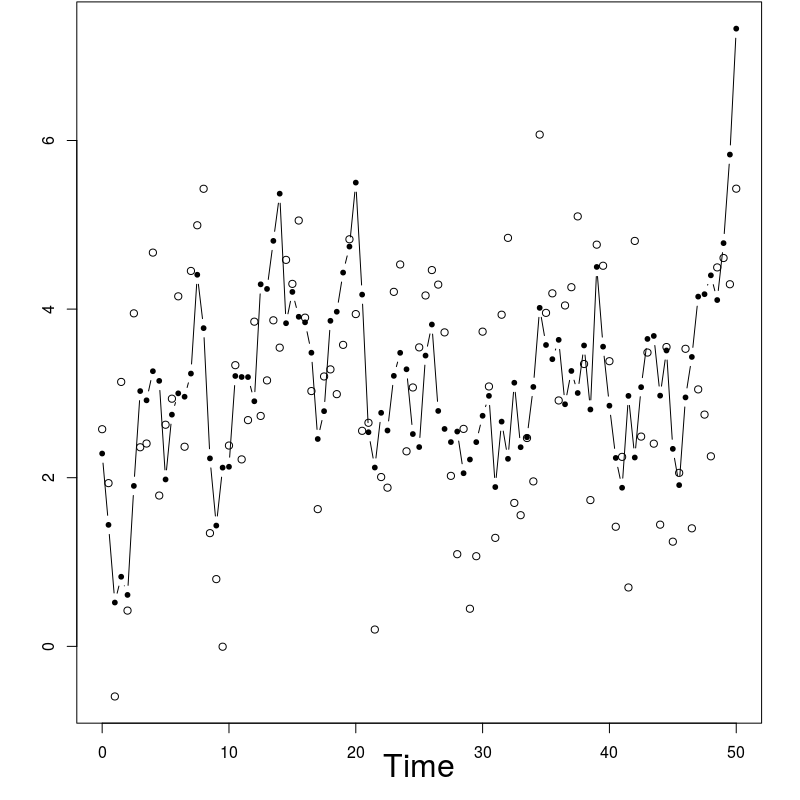
\includegraphics[scale = .5]{obs_SINE}
\caption{{\em SINE model - observations}. Process $X$ solution to the SDE (balls) and observations $Y$ (circles) at times $t_0=0,\dots,t_{100}=50$.}
\label{fig:res:SINE:obs}
\end{figure}

\begin{figure}[p]
\centering
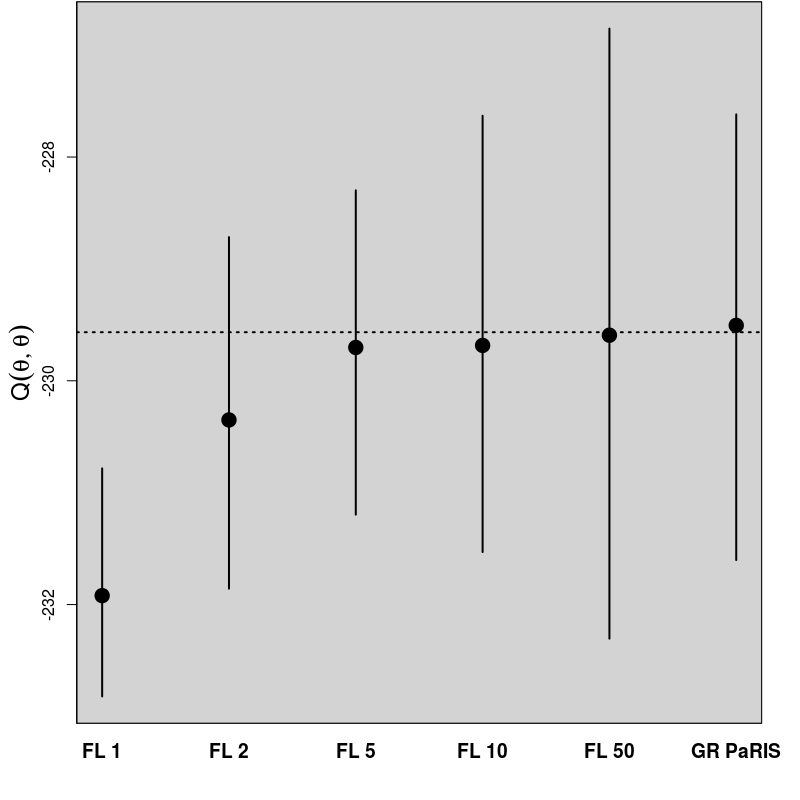
\includegraphics[scale=0.5]{res_Estep_SINE}
\caption{{\em SINE model - EM intermediate quantity}. Estimation of the EM intermediate quantity $\mathcal{Q}(\theta,\theta)$  using the fixed lag (FL) technique for 5 different lags, and the GRand PaRIS algorithm using 200 replicates. 
The whiskers represent the extent of the 95\% central values. 
The dot represents the empirical mean over the 200 replicates. 
The dotted line shows the reference value, computed using the GRand PaRIS algorithm with $N = 5000$ particles.}
\label{fig:res:SINE:EM}
\end{figure}


\begin{figure}[p]
\centering
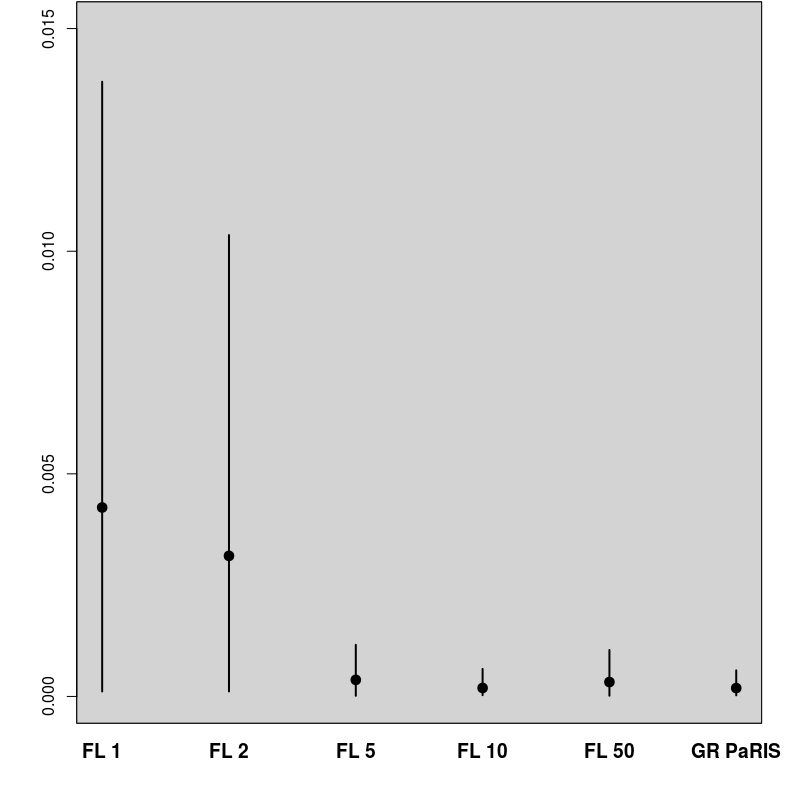
\includegraphics[scale=0.5]{res_mult_SINE_bias}
\caption{{\em SINE model - bias}. Distribution of the empirical absolute relative bias.}
\label{fig:mult:SINE:b}
\end{figure}

\begin{figure}[p]
\centering
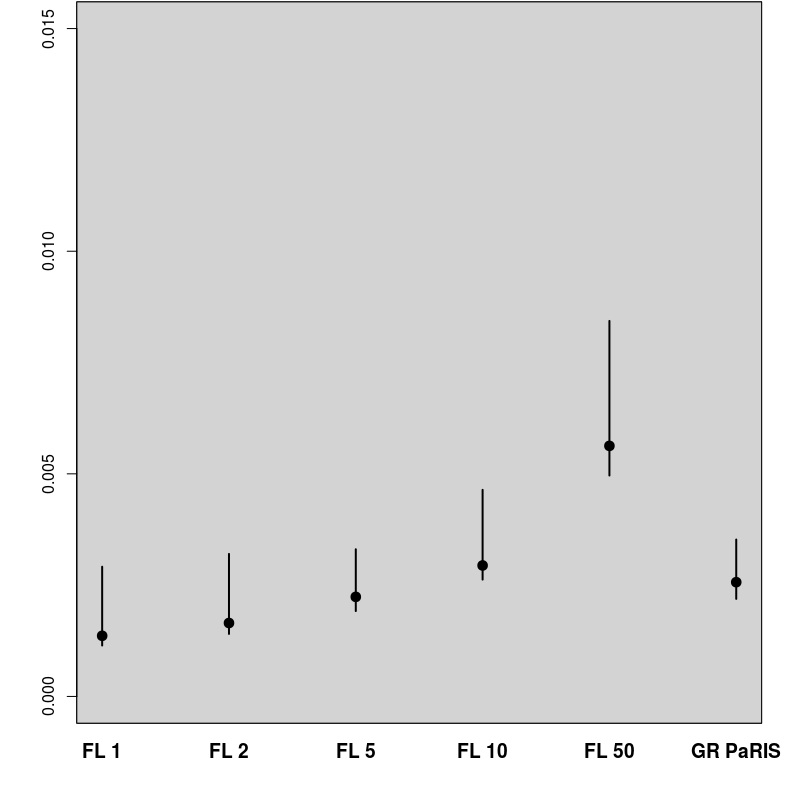
\includegraphics[scale=0.5]{res_mult_SINE_cv}
\caption{{\em SINE model - variance}. Distribution of the empirical absolute coefficient of variation.}
\label{fig:mult:SINE:cv}
\end{figure}
\paragraph{Generalized EM procedure}
The performance of our algorithm is also assessed in the case where $\theta$ and the variance $\sigma^2_\text{obs}$ are unknown and estimated using a generalized EM algorithm. 
The study is done using a data set with $n = 200$ observations simulated with $\mu=0$ an d $ \sigma^2_\text{obs} = 1$. The Grand PaRIS algorithm is used to perform the E step, with the same settings as before for $N$, $\tilde{N}$ and $M$.
As there is no closed form solution to compute the M step of the EM algorithm and propose new parameter estimates, we use a Generalized EM procedure: given the current estimation $\theta^{(k)} := \left(\mu^{(k)}, \sigma_{\text{obs}}^{(k)} \right)$, the function $\mathcal{Q}(\cdot, \theta^{(k)})$ is approximated for $50$ new candidates $\theta_1, \dots, \theta_{50} $ chosen by the user. The new estimate is set as
\[
\theta^{(k + 1)} = \text{argmax}_i\mathcal{Q}(\theta_i, \theta^{(k)})\eqsp .
\]
This procedure has the nice property of using the same particle filter and the same retrospective sampling of Lemma \ref{lem:AR:unbiased} for all candidates, avoiding to repeat this time consuming procedure. 
The number of candidates and the way to choose them is problem dependent and then left to the user. 
In our case, we sampled candidates using Gaussian distributions around the currend estimate $\theta^{(k)}$, decreasing the variance when $k$ increases.
Figures~\ref{fig:SINE:theta} and~\ref{fig:SINE:sigma} illustrate the performance of the estimation for 12 different initializations of $\mu$ (resp. $\sigma_\text{obs}$) uniformly chosen in  $]-\pi,\pi[$ (resp. in $]0,6[$), illustrating a convergence after only a few iterations of the EM procedure.

\begin{figure}[p]
\centering
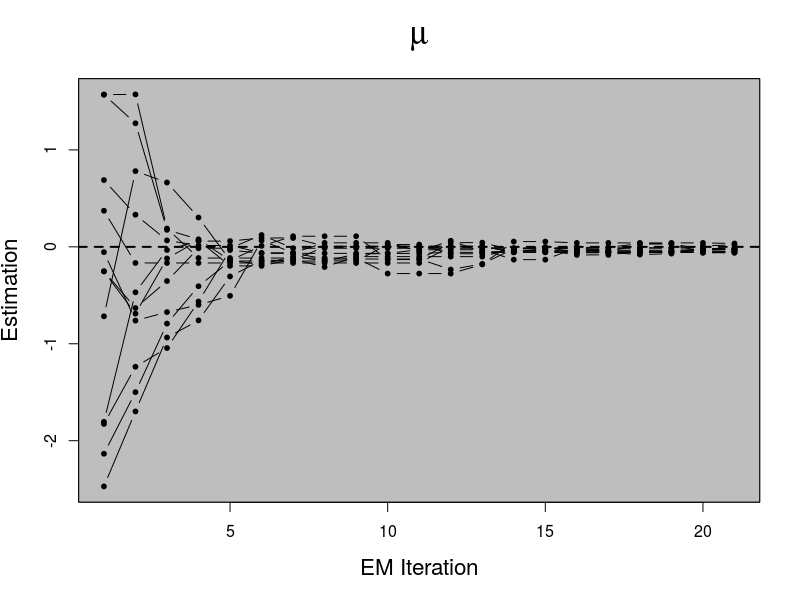
\includegraphics[scale=0.5]{figure_theta}
\caption{{\em SINE model - EM}. Estimation  of $\mu$.}
\label{fig:SINE:theta}
\end{figure}


\begin{figure}[p]
\centering
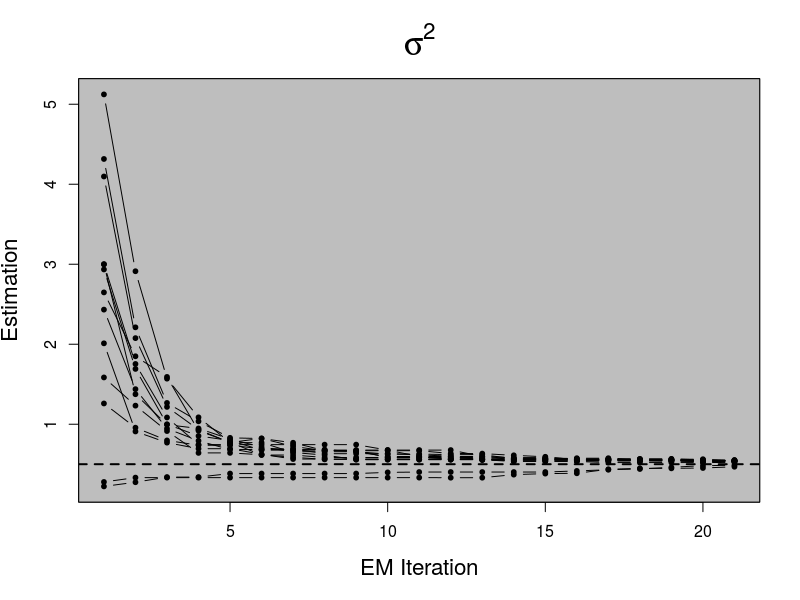
\includegraphics[scale=0.5]{figure_sigma2}
\caption{{\em SINE model - EM}. Estimation of $\sigma_\text{obs}$.}
\label{fig:SINE:sigma}
\end{figure}


\subsection*{Log-growth model}
Following \cite{beskos:papaspiliopoulos:roberts:fearnhead:2006} and \cite{olsson:westerborn:2016}, the performance of the proposed algorithm are also illustrated with the log-growth model defined by:
\begin{equation}
\rmd Z_t = \kappa Z_t\left(1-\frac{Z_t}{\gamma}\right)\rmd t + \sigma Z_t \rmd W_t,~~Z_0=z_0\eqsp . \label{eq:LG:SDE}
\end{equation}
In order to use the exact algorithms of \cite{beskos:papaspiliopoulos:roberts:fearnhead:2006} and the GPE of \cite{fearnhead:papaspiliopoulos:roberts:2008}, we consider  \eqref{eq:LG:SDE} after the Lamperti transform, i.e., the process defined by $X_t=\eta(Z_t)$, with $\eta(z) := -\log (z)/\sigma$,  which satisfies the following SDE:
\begin{equation}
\rmd X_t = \overbrace{\left( \frac{\sigma}{2} -  \frac{\kappa}{\sigma} + \frac{\kappa}{\gamma\sigma}\exp\left(-\sigma X_t\right)\right)}^{:=\alpha(X_t)}\rmd t +\rmd W_t,~~X_0=x_0=\eta(z_0)\eqsp.\label{eq:Lamp:LG}
\end{equation}
In this case, the conditions of the Exact Algorithm~2 defined in \cite{beskos:papaspiliopoulos:roberts:fearnhead:2006} are satisfied, as for any $m \in \mathbb{R}$ there exists $\mathsf{U}_m$ such that for all $x\ge m$, $\psi(x):=\alpha^2(x)+\alpha'(x) \leq \mathsf{U}_m$. Moreover, $\psi$ is lower bounded uniformly by  $\mathsf{L}$. 
Then, GPE estimators may be computed by simulating the minimum of a Brownian bridge, and simulating Bessel bridges conditionally to this minimum, as proposed by \cite{beskos:papaspiliopoulos:roberts:fearnhead:2006}.

The process solution to \eqref{eq:Lamp:LG} is observed regularly at times $t_0=0,\dots,t_{50}=100$ through the observation process $(Y_k)_{0\le k\le 50}$ defined as:
\begin{equation*}
Y_k = X_k + \varepsilon_k\eqsp,
\end{equation*}
where the $(\varepsilon_k)_{0\le k \le 50}$ are i.i.d. $ \mathcal{N}(0,\sigma^2_{obs})$.
The parameters are given by $$\theta =(\kappa=0.1,\sigma=0.1,\gamma=1000,\sigma_{obs} = 2)\eqsp.$$
In the case of the Log-growth model, the estimator $\widehat{q}_k(\cdot)$ defined by equation \eqref{eq:GPE1} satisfies \eqref{assumpt:ysupport}, leading to a GRand PaRIS algorithm with linear complexity in the number of particles. However, the remarks about the bound $\widehat{\sigma}_+^k$
 made for the SINE model above still hold in this case.  
The intermediate quantity of the EM algorithm is evaluated  as for the SINE model, see Figures~\ref{fig:res:LG:EM},~\ref{fig:mult:LG:b} and~\ref{fig:mult:LG:cv}.

The results for the fixed lag technique are similar to the ones presented in \cite[Figure 1]{olsson:strojby:2011} using the same model. 
For small lags, the variance of the estimates is small, but the estimation is highly biased. 
The bias rapidly decreases as the lag increases, together with a  great increase of variance.  
Again, the GRand PaRIS algorithm outperforms the fixed lag smoother as it shows  a similar (vanishing) bias as the fixed lag for the largest lag and a smaller variance than the fixed lags estimates with negligible bias. 

Note that in this case the Lamperti transform to obtain a diffusion with a unitary diffusion term depends on $\sigma$. 
The process $(X_t)_{t\ge 0}$ is a function of $\sigma$ and is not directly observed if $\sigma$ is unknown, which prevents a direct use of an EM algorithm to estimate $\sigma$. 
Following \cite[Section~8.2]{beskos:papaspiliopoulos:roberts:fearnhead:2006}, this may be overcome with a two-step transformation of the process $(Z_t)_{t\ge 0}$.
\begin{figure}[p]
\centering
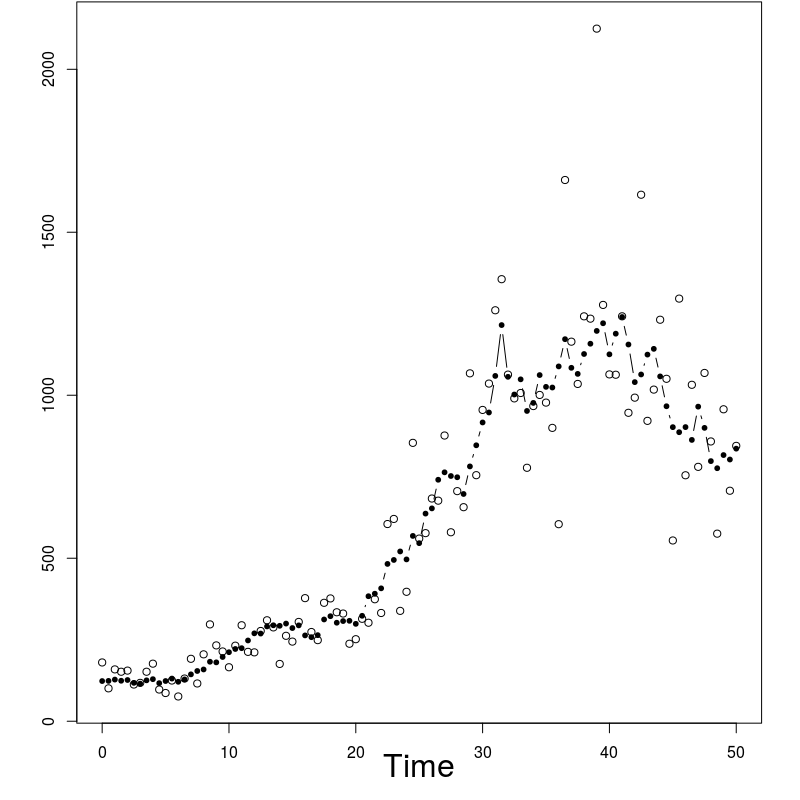
\includegraphics[scale=0.5]{obs_LG}
\caption{{\em Log-growth model - observations}.
 Process $X$ solution to the SDE (balls) and observations $Y$ (circles) at times $t_0=0,\dots,t_{100}=50$.}
\label{fig:res:LG:obs}
\end{figure}

\begin{figure}[p]
\centering
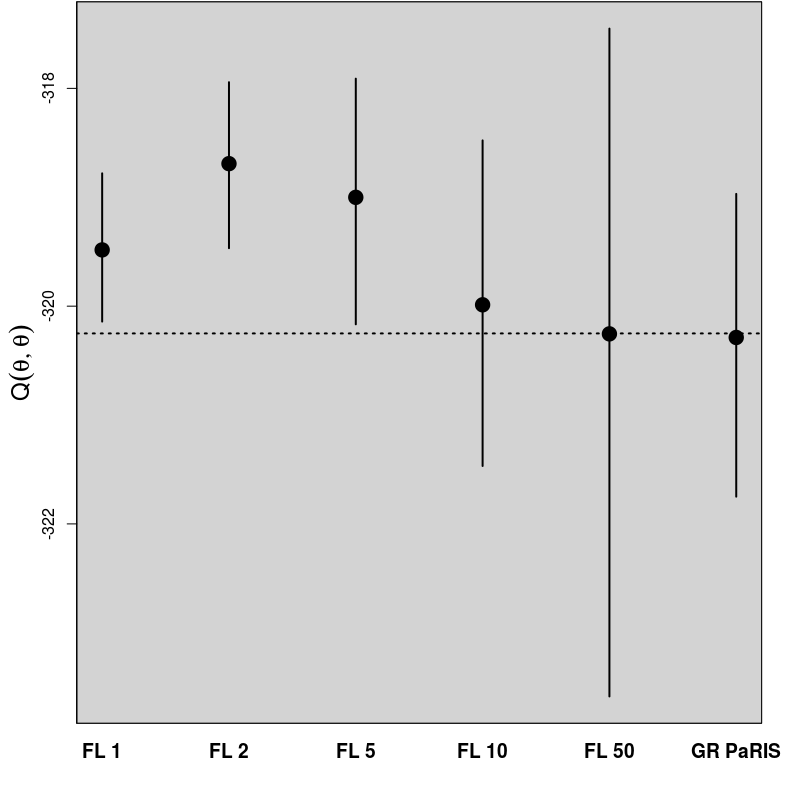
\includegraphics[scale=0.5]{res_Estep_LG}
\caption{{\em Log-growth model - EM intermediate quantity}.
 Estimation of the EM intermediate quantity $\mathcal{Q}(\theta,\theta)$  using the fixed lag (FL) technique for 5 different lags, and the GRand PaRIS algorithm using 200 replicates.
  The whiskers represent the extent of the 95\% central values. The dot represents the empirical mean over the 200 replicates.
   The dotted line shows the reference value, computed using the GRand PaRIS algorithm with $N=5000$ particles.}
\label{fig:res:LG:EM}
\end{figure}


\begin{figure}[p]
\centering
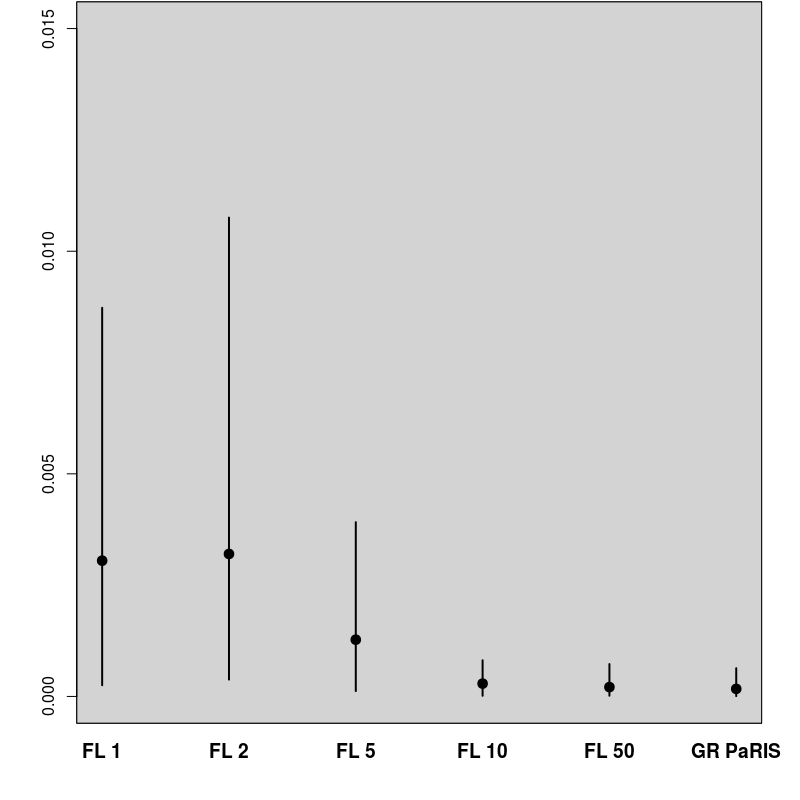
\includegraphics[scale=0.5]{res_mult_LG_bias}
\caption{{\em Log-growth model - biais}. 
Distribution of the empirical absolute relative bias.}
\label{fig:mult:LG:b}
\end{figure}

\begin{figure}[p]
\centering
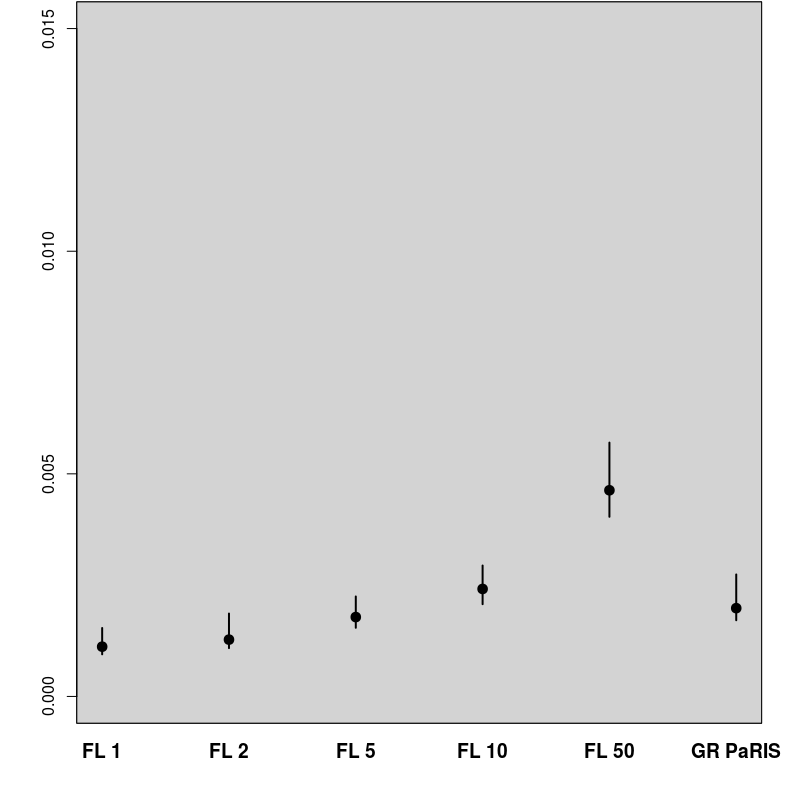
\includegraphics[scale=0.5]{res_mult_LG_cv}
\caption{{\em Log-growth model - variance}.
 Distribution of the empirical absolute coefficient of variation.}
\label{fig:mult:LG:cv}
\end{figure}

\section{Conclusions}
This paper presents a new online SMC smoother for partially observed differential equations.
 This algorithm relies on an acceptance-rejection procedure inspired from the recent PaRIS algorithm.
 The main result of the article for practical applications is that the mechanism of this procedure remains valid when the transition density is approximated by a an unbiased positive estimator.
  The proposed procedure therefore extends the PaRIS algorithm to HMMs whose transition density is unknown and can be unbiasedly approximated. The GRand PaRIS algorithm outperforms the existing fixed lag smoother for POD processes of \cite{olsson:strojby:2011}, as it does not introduce any intrinsic and non vanishing bias.
   In addition, numerical simulations highlight a better variance using data from two different models.
   It can be implemented for the class of models for which exact algorithms of \cite{beskos:papaspiliopoulos:roberts:fearnhead:2006} are valids, with a linear complexity in $N$ in the best cases, or at worse in $N^2$. 

\subsection*{Competing interests}
The authors have no competing interests. 

\subsection*{Funding}
This work has been developed during a one year postdoc funded by Paris-Saclay Center for Data Science. 

\subsection*{Authors' contributions}
All the authors have contributed to the conception of the algorithms, the analysis of the proposed estimator and to the redaction of the manuscript.
 Pierre Gloaguen provided the simulations displayed in the final version. 

\appendix

\section{Proofs}
\label{sec:append:proofs}
\begin{proof}[Proof of Lemma~\ref{lem:AR:unbiased}]
Let $\tau$ be the first time  draws are accepted in the accept-reject mechanism. For all $\ell\ge 1$, write
\[
\mathcal{A}^k_{\ell} = \left\{U_\ell<\widehat{q}_{k}(\xi_{k}^{J_\ell},\xi_{k+1}^{i},\zeta^{\ell}_{k})/\hat{\sigma}^k_+\right\}\eqsp.
\]
Let $h$ be a function defined on $\{1,\ldots,N\}$,
\begin{align*}
\mathbb{E}\left[h(J^{i,j}_k)\middle| \mathcal{G}_{k+1}^N\right] & = \sum_{m\ge 1}\mathbb{E}\left[h(J_m)\1_{\tau=m}\middle| \mathcal{G}_{k+1}^N\right]\eqsp,\\
& = \sum_{m\ge 1}\left(\prod_{\ell=1}^{m-1}\mathbb{E}\left[\1_{(\mathcal{A}^k_{\ell})^c}\middle| \mathcal{G}_{k+1}^N\right]\right)\mathbb{E}\left[h(J_m)\1_{\mathcal{A}^k_{m}}\middle| \mathcal{G}_{k+1}^N\right]\eqsp,\\
& = \sum_{m\ge 1}\left(\prod_{\ell=1}^{m-1}\mathbb{E}\left[1-\frac{\widehat{q_k}(\xi_{k}^{J_\ell},\xi_{k+1}^{i};\zeta_k^{\ell})}{\hat{\sigma}^k_{+}}\middle| \mathcal{G}_{k+1}^N\right]\right)\\
&\hspace{5cm}\times\mathbb{E}\left[h(J_m)\frac{\widehat{q_k}(\xi_{k}^{J_m},\xi_{k+1}^{i};\zeta_k^{m})}{\hat{\sigma}^k_{+}}\middle| \mathcal{G}_{k+1}^N\right]\eqsp,\\
& = \sum_{m\ge 1}\left(\mathbb{E}\left[1-\frac{q_k(\xi_{k}^{J_1},\xi_{k+1}^{1})}{\hat{\sigma}^k_{+}}\middle| \mathcal{G}_{k+1}^N\right]\right)^{m-1}\mathbb{E}\left[h(J_1)\frac{q_k(\xi_{k}^{J_1},\xi_{k+1}^{1})}{\hat{\sigma}^k_{+}}\middle| \mathcal{G}_{k+1}^N\right]\eqsp,\\
& = \mathbb{E}\left[h(J_1)q_k(\xi_{k}^{J_1},\xi_{k+1}^{i})\middle| \mathcal{G}_{k+1}^N\right]/\mathbb{E}\left[q_k(\xi_{k}^{J_1},\xi_{k+1}^{i})\middle| \mathcal{G}_{k+1}^N\right]\eqsp,\\
& = \sum_{\ell=1}^N \frac{h(\ell)\omega_{k-1}^{\ell}q_k(\xi_{k}^{\ell},\xi_{k+1}^{i})}{\sum_{m=1}^N\omega_{k-1}^{m}q_k(\xi_{k}^{m},\xi_{k+1}^{i})}\eqsp,\\
&= \sum_{\ell=1}^N \Lambda_{k-1}^N(i,\ell)h(\ell) \eqsp,
\end{align*}
which concludes the proof.
\end{proof}


\begin{proof}[Proof of Lemma \ref{lem:iid}]
The independence is ensured by the mechanism of SMC methods. By \eqref{eq:random:weight},
\[
\mathbb{E}\left[\widehat{\omega}^i_{k+1}\tau^{i}_{k+1}\middle| \mathcal{F}_k^{N}\right] = \mathbb{E}\left[\frac{ \widehat{\qk}(\xi_{k}^{I^{i}_{k+1}}, \xi^{i}_{k+1};\zeta_{k})g_{k+1}(\xi^{i}_{k+1})}{\vartheta_{k+1}(\xi^{I^{i}_{k+1}}_{k}) p_{k}(\xi_{k}^{I^{i}_{k+1}},\xi^{i}_{k+1})}\tau^{i}_{k+1}\middle| \mathcal{F}_k^{N}\right]\eqsp.
\]
Note that by Lemma~\ref{lem:AR:unbiased},
\begin{align*}
&\mathbb{E}\left[\tau^{i}_{k+1}\middle|\mathcal{G}_{k+1}^{N}\right]
 = \sum_{\ell=1}^N\frac{\omega_k^{\ell} \qk(\xi_{k}^{\ell}, \xi^{i}_{k+1}) \left(\tau^{\ell}_k + h_{k}(\xi_{k}^{\ell},\xi^{i}_{k+1})\right)}{\sum_{\ell'=1}^N\omega_k^{\ell'} \qk(\xi_{k}^{\ell'},\xi^{i}_{k+1})}\eqsp,\\
&\mathbb{E} \left[\widehat{\qk}(\xi_{k}^{I^{i}_{k+1}},\xi^{i}_{k+1};\zeta_{k}) \middle| \mathcal{G}_{k+1}^{N}\right]
 = \qk(\xi_{k}^{I^{i}_{k+1}},\xi^{i}_{k+1})\eqsp.
\end{align*}
Since $\tau^{i}_{k+1}$ and $\zeta_{k}$ are independent conditionally to $\mathcal{G}_{k+1}^{N}$:
\begin{multline*}
\mathbb{E}\left[\tau^{i}_{k+1} \widehat{\qk} (\xi_{k}^{I^{i}_{k+1}},\xi^{i}_{k+1};\zeta_{k})\middle|\mathcal{G}_{k+1}^{N}\right]\\
 = q_k(\xi_{k}^{I^{i}_{k+1}},\xi^{i}_{k+1})\sum_{\ell=1}^N\frac{\omega_k^{\ell} \qk (\xi_{k}^{\ell},\xi^{i}_{k+1})\left(\tau^{\ell}_k + h_{k}(\xi_{k}^{\ell},\xi^{i}_{k+1})\right)}{\sum_{\ell'=1}^N\omega_k^{\ell'} \qk (\xi_{k}^{\ell'},\xi^{i}_{k+1})}\eqsp.
\end{multline*}
Moreover, conditionally to $\mathcal{F}_k^N$, the probability density function of $(\xi_{k+1}^i,I_{k+1}^i)$ is given by
\[
(x,j) \mapsto \frac{\omega_k^j\vartheta_{k+1}(\xi_k^j)p_k(\xi_k^j,x)}{\Omega_k\phi_k^N[\vartheta_{k+1}]}\eqsp.
\]
Therefore, this yields:
\begin{align*}
\mathbb{E}\left[\widehat{\omega}^i_{k+1}\tau^{i}_{k+1}\middle| \mathcal{F}_k^{N}\right]&= \left(\phi^N_{k}[\vartheta_{k+1}]\right)^{-1} \sum_{j=1}^N\frac{\omega_k^j}{\Omega_k} \int \vartheta_{k+1}(\xi^{j}_{k})\frac{\qk(\xi_{k}^{j},x) g_{k+1}(x)}{\vartheta_{k+1}(\xi^{j}_{k}) p_{k}(\xi_{k}^{j},x)}\\
&\hspace{1cm}\times \sum_{\ell=1}^N\frac{\omega_k^{\ell} \qk (\xi_{k}^{\ell},x)\left(\tau^{\ell}_k + h_{k}(\xi_{k}^{\ell},x)\right)}{\sum_{\ell'=1}^N\omega_k^{\ell'}\qk(\xi_{k}^{\ell'},x)}p_{k}(\xi_{k}^{j},x)\rmd x\eqsp,\\
&= \left(\phi^N_{k}[\vartheta_{k+1}]\right)^{-1}\\
&~~~~\times\sum_{\ell=1}^N \frac{\omega_k^\ell}{\Omega_k}\left[\int \frac{ \sum_{j=1}^N \omega_k^j\qk(\xi_k^j,x) }{ \sum_{\ell'=1}^N\omega_k^{\ell'}\qk(\xi_{k}^{\ell'},x) } g_{k+1}(x)\qk (\xi_{k}^{\ell},x)\left(\tau^{\ell}_k + h_{k}(\xi_{k}^{\ell},x)\right) \rmd x \right]\\ 
& =\left(\phi^N_{k}[\vartheta_{k+1}]\right)^{-1}\phi^N_{k}\left[\int \qk(\cdot,x)g_{k+1}(x)\left\{\tau_k(\cdot) + h_{k}(\cdot,x)\right\}\rmd x\right]\eqsp,
\end{align*}
which concludes the proof.
\end{proof}


\begin{proof}[Proof of Proposition~\ref{prop:exp:deviation}]
The results is proved by induction. At time $k=0$, the result holds using that for all $1\le i \le N$, $\rho_0^i = 0$ and the convention $T_0[h_0] =0$. In addition, $\phi_0^N$ is a standard importance sampler estimator of $\phi_0$ with $\widehat \omega_0^i\le |\widehat{\omega}_0|_{\infty}$ so that for any bounded function $h$ on $\mathsf{X}$,
\[
\mathbb{P}\left(\left|\phi_0^N[h] - \phi_0\left[h\right]\right|\ge \varepsilon\right)\le b_0\exp\left(-c_0N\varepsilon^2\right)\eqsp.
\]
Assume the results holds for $k\ge 1$ and that $\vartheta_{k+1} = 1$ for simplicity. Write
\[
\phi_{k+1}^N[\tau_{k+1}] - \phi_{k+1}\left[T_{k+1}[h_{k+1}]\right] = a_N/b_N\eqsp,
\]
where $a_N = N^{-1}\sum_{i=1}^N \widehat{\omega}_{k+1}^i \left(\tau_{k+1}^i - \phi_{k+1}\left[T_{k+1}[h_{k+1}]\right]\right)$ and $b_N =N^{-1}\sum_{i=1}^N \widehat{\omega}_{k+1}^i$. By Lemma~\ref{lem:iid}, the random variables $\{\widehat{\omega}_{k+1}^i\tau_{k+1}^i\}_{i=1}^N$ are independent conditionally on $\mathcal{F}_k^{N}$ and by H\ref{assum:boundalgo},
\[
\left|\widehat{\omega}_{k+1}^i \left(\tau_{k+1}^i - \phi_{k+1}\left[T_{k+1}[h_{k+1}]\right]\right)\right| \le 2|\widehat{\omega}_{k+1}|_{\infty}|H_{k+1}|_{\infty}\eqsp.
\]
Therefore, by Hoeffding inequality,
\[
\mathbb{P}\left(\left|a_N - \mathbb{E}\left[a_N\middle|\mathcal{F}_k^{N}\right]\right|\ge \varepsilon\right) = \mathbb{E}\left[\mathbb{P}\left(\left|a_N - \mathbb{E}\left[a_N\middle|\mathcal{F}_k^{N}\right]\right|\ge \varepsilon\middle|\mathcal{F}_k^{N}\right)\right]\le 2\exp\left(-c_kN\varepsilon^2\right)\eqsp.
\] 
On the other hand,
\[
%\mathbb{E}\left[a_N\middle|\mathcal{F}_k^{N}\right] = \left(\phi^N_{k}[\vartheta_{k+1}]\right)^{-1}\phi^N_{k}\left[\Upsilon_k\right] \eqsp,
\mathbb{E}\left[a_N\middle|\mathcal{F}_k^{N}\right] = \phi^N_{k}\left[\Upsilon_k\right] \eqsp,
\]
where
\[
\Upsilon_k(x_k) = \int q_{k}(\cdot,x)g_{k+1}(x)\left(\tau_k(x_k) + h_{k+1}(x_k,x) - \phi_{k+1}\left[T_{k+1}[h_{k+1}]\right]\right)\rmd x\eqsp.
\]
By \cite[Lemma~11]{olsson:westerborn:2016}, $\phi_{k}\left[\Upsilon_k\right] = 0$ which implies by the induction assumption that 
\[
\mathbb{P}\left(\left|\mathbb{E}\left[a_N\middle|\mathcal{F}_k^{N}\right]\right|\ge \varepsilon\right)\le b_k\exp\left(-c_kN\varepsilon^2\right)\eqsp.
\]
Then,
\[
\mathbb{P}\left(\left|a_N\right|\ge \varepsilon\right) \le b_k\exp\left(-c_kN\varepsilon^2\right)\eqsp.
\] 
Similarly, as $b_N \le |\widehat{\omega}_k|_{\infty}$, by Hoeffding inequality,
\begin{multline*}
\mathbb{P}\left(\left|b_N - \mathbb{E}\left[b_N\middle|\mathcal{F}_k^{N}\right]\right|\ge \varepsilon\right) \\
= \mathbb{E}\left[\mathbb{P}\left(\left|b_N - \mathbb{E}\left[b_N\middle|\mathcal{F}_k^{N}\right]\right|\ge \varepsilon\middle|\mathcal{F}_k^{N}\right)\right]\le 2\exp\left(-c_kN\varepsilon^2\right)\eqsp.
\end{multline*}
Note that
\[
\mathbb{E}\left[b_N\middle|\mathcal{F}_k^{N}\right] = \phi^N_{k}\left[\int q_{k}(\cdot,x)g_{k+1}(x)\rmd x\right]\eqsp.
\]
By  the induction assumption,
\[
\mathbb{P}\left(\left|\mathbb{E}\left[b_N\middle|\mathcal{F}_k^{N}\right]-\phi_k\left[\int q_{k}(\cdot,x)g_{k+1}(x)\rmd x\right]\right|\ge \varepsilon\right)\le b_k\exp\left(-c_kN\varepsilon^2\right)\eqsp.
\]
The proof is completed using Lemma~\ref{lem:hoeffding:ratio}.
\end{proof}


\begin{lemma}\label{lem:hoeffding:ratio}
Assume that $a_N$, $b_N$, and $b$ are random variables defined on the same probability space such that there exist positive constants $\beta$, $B$, $C$, and $M$ satisfying
\begin{enumerate}[(i)]
    \item $|a_N/b_N|\leq M$, $\mathbb{P}$-a.s.\ and  $b \geq \beta$, $\mathbb{P}$-a.s.,
    \item For all $\epsilon>0$ and all $N\geq1$, $\mathbb{P}\left[|b_N-b|>\epsilon \right]\leq B \exp\left(-C N \epsilon^2\right)$,
    \item For all $\epsilon>0$ and all $N\geq1$, $\mathbb{P} \left[ |a_N|>\epsilon \right]\leq B \exp\left(-C N \left(\epsilon/M\right)^2\right)$.
\end{enumerate}
Then,
$$
    \mathbb{P}\left\{ \left| \frac{a_N}{b_N} \right| > \epsilon \right\} \leq B \exp{\left(-C N \left(\frac{\epsilon \beta}{2M} \right)^2 \right)} \eqsp.
$$
\end{lemma}
\begin{proof}
See \cite{douc:garivier:moulines:olsson:2011}.
\end{proof}



\bibliographystyle{plain}
%\bibliography{Paris_EM}
\begin{thebibliography}{10}

\bibitem{ait-sahalia:1999}
Y.~Ait-Sahalia.
\newblock Transition densities for interest rate and other nonlinear
  diffusions.
\newblock {\em Journal of {Finance}}, 54:1361--1395, 1999.

\bibitem{ait-sahalia:2002}
Y.~Ait-Sahalia.
\newblock Maximum likelihood estimation of discretely sampled diffusions: a
  closed-form approximation approach.
\newblock {\em Econometrica}, 70:223--262, 2002.

\bibitem{ait-sahalia:2008}
Y.~Ait-Sahalia.
\newblock Closed-form likelihood expansions for multivariate diffu- sions.
\newblock {\em The {A}nnals of {S}tatistics}, 36:906--937, 2008.

\bibitem{beskos:papaspiliopoulos:roberts:2006}
A.~Beskos,  O.~Papaspiliopoulos, and G.O.~Roberts.
\newblock Retrospective exact simulation of diffusion sample paths with applications.
\newblock {\em Bernoulli}, 12(6):1077:1098, 2006.

\bibitem{beskos:papaspiliopoulos:roberts:2008}
A.~Beskos, O.~Papaspiliopoulos, G.O.~Roberts.
\newblock A factorisation of diffusion measure and finite sample path constructions.
\newblock {\em Methodology and {C}omputing in {A}pplied {P}robability}, 10(1):85--104, 2008.

\bibitem{beskos:papaspiliopoulos:roberts:fearnhead:2006}
A.~Beskos, O.~Papaspiliopoulos, G.O.~Roberts, and P.~Fearnhead.
\newblock Exact and computationally efficient likelihood-based estimation for
  discretely observed diffusion processes (with discusion).
\newblock {\em J. Roy. Statist. Soc. Ser. B}, 68(3):333--382, 2006.

\bibitem{cappe:moulines:ryden:2005}
O.~Capp\'{e}, E.~Moulines, and T.~Ryd\'{e}n.
\newblock {\em Inference in Hidden {M}arkov Models}.
\newblock Springer, 2005.

\bibitem{delmoral:jacod:protter:2001}
P.~Del~Moral, J.~Jacod, and P.~Protter.
\newblock The {M}onte {C}arlo method for filtering with discrete-time
  observations.
\newblock {\em Probability {T}heory and {R}elated {F}ields}, 120:346 -- 368,
  2001.

\bibitem{dempster:laird:rubin:1977}
A.~P. Dempster, N.~M. Laird, and D.~B. Rubin.
\newblock Maximum likelihood from incomplete data via the {EM} algorithm.
\newblock {\em J. Roy. Statist. Soc. B}, 39(1):1--38 (with discussion), 1977.

\bibitem{douc:garivier:moulines:olsson:2011}
R.~Douc, A.~Garivier, E.~Moulines, and J.~Olsson.
\newblock Sequential {M}onte {C}arlo smoothing for general state space hidden
  {M}arkov models.
\newblock {\em Ann. Appl. Probab.}, 21(6):2109--2145, 2011.

\bibitem{doucet:godsill:andrieu:2000}
A.~Doucet, S.~Godsill, and C.~Andrieu.
\newblock On sequential {M}onte-{C}arlo sampling methods for {B}ayesian
  filtering.
\newblock {\em Stat. Comput.}, 10:197--208, 2000.

\bibitem{doucetgodsillandrieu:2000}
A.~Doucet, S.~Godsill, and C.~Andrieu.
\newblock On sequential monte-carlo sampling methods for bayesian filtering.
\newblock {\em Statistics and Computing}, 10:197 -- 208, 2000.

\bibitem{fearnhead:papaspiliopoulos:roberts:2008}
P.~Fearnhead, O.~Papaspiliopoulos, and G.O.~Roberts.
\newblock Particle filters for partially observed diffusions.
\newblock {\em J. Roy. Statist. Soc. Ser. B}, 70(4):755--777, 2008.

\bibitem{fearnhead:latuszynski:roberts:sermaidis:2017}
P.~Fearnhead, K.~Latuszynski, G.O.~Roberts and G.~Sermaidis.
\newblock Continuous-time Importance Sampling: {M}onte {C}arlo methods which avoid time-discretisation error.
\newblock {\em Technical report}, 2017.

\bibitem{gloaguen:etienne:lecorff:2017}
P.~ Gloaguen, M.-P.~\'Etienne, and S.~Le~Corff.
\newblock Stochastic differential equation based on a multimodal potential to model movement data in ecology\textit{•}.
\newblock {\em To appear in the {J}ournal of the {R}oyal {S}tatistical {S}ociety: {S}eries {C}}.

\bibitem{godsill:doucet:west:2004}
S.~J. Godsill, A.~Doucet, and M.~West.
\newblock {M}onte {C}arlo smoothing for non-linear time series.
\newblock {\em J. Am. Statist. Assoc.}, 50:438--449, 2004.

\bibitem{gordon:salmond:smith:1993}
N.~Gordon, D.~Salmond, and A.F. Smith.
\newblock Novel approach to nonlinear/non-{G}aussian bayesian state estimation.
\newblock {\em {IEE} Proc. {F}, Radar Signal Process}, 140:107--113, 1993.

\bibitem{huerzeler:kunsch:1998}
M.~H{\"u}rzeler and H.~R. K{\"u}nsch.
\newblock {M}onte {C}arlo approximations for general state-space models.
\newblock {\em J. Comput. Graph. Statist.}, 7:175--193, 1998.

\bibitem{kantas:doucet:signh:2015}
N.~Kantas, A.~Doucet, S.S. Singh, J.~Maciejowski, and N.~Chopin.
\newblock On particle methods for parameter estimation in state-space models.
\newblock {\em Statist. Sci.}, 30(3):328--351, 2015.

\bibitem{kessler:1997}
M.~Kessler.
\newblock Estimation of an ergodic diffusion from discrete observations.
\newblock {\em Scandinavian Journal of Statistics}, 24(2):211--229, 1997.

\bibitem{kessler:lindner:sorensen:2012}
M.~Kessler, A.~Lindner, and M.~Sorensen.
\newblock {\em Statistical methods for stochastic differential equations}.
\newblock CRC Press, 2012.

\bibitem{kitagawa:1996}
G.~Kitagawa.
\newblock {M}onte-{C}arlo filter and smoother for non-{G}aussian nonlinear
  state space models.
\newblock {\em J. Comput. Graph. Statist.}, 1:1--25, 1996.

\bibitem{lecorff:fort:2013a}
S.~Le~Corff and G.~Fort.
\newblock Convergence of a particle-based approximation of the block online
  {E}xpectation {M}aximization algorithm.
\newblock {\em ACM Transactions on Modeling and Computer Simulation}, 23(1):2,
  2013.

\bibitem{lecorff:fort:2013b}
S.~Le~Corff and G.~Fort.
\newblock Online {E}xpectation {M}aximization based algorithms for inference in
  hidden {M}arkov models.
\newblock {\em Electronic Journal of Statistics}, 7:763--792, 2013.

\bibitem{li:2013}
C.~Li.
\newblock Maximum-likelihood estimation for diffusion processes via closed-form
  density expansions.
\newblock {\em The {A}nnals of {S}tatistics}, 41(3):1350--1380, 2013.

\bibitem{olsson:cappe:douc:moulines:2008}
J.~Olsson, O.~Cappe, R.~Douc, and E.~Moulines.
\newblock Sequential monte carlo smoothing with application to parameter
  estimation in nonlinear state space models.
\newblock {\em Bernoulli}, 14(1):155--179, 2008.

\bibitem{olsson:strojby:2011}
J.~Olsson and J.~Strojby.
\newblock Particle-based likelihood inference in partially observed diffusion
  processes using generalised {P}oisson estimators.
\newblock {\em Electron. J. Statist.}, 5:1090--1122, 2011.

\bibitem{olsson:westerborn:2016}
J.~Olsson and J.~Westerborn.
\newblock Efficient particle-based online smoothing in general hidden {M}arkov
  models: the {PaRIS} algorithm.
\newblock {\em Bernoulli}, 3:1951--1996, 2017 .

\bibitem{ozaki:1992}
T.~Ozaki.
\newblock A bridge between nonlinear time series models and nonlinear
  stochastic dynamical systems: a local linearization approach.
\newblock {\em Statistica Sinica}, 2:1130--135, 1992.

\bibitem{pitt:shephard:1999}
M.K. Pitt and N.~Shephard.
\newblock Filtering via simulation: Auxiliary particle filters.
\newblock {\em J. Am. Statist. Assoc.}, 94(446):590--599, 1999.

\bibitem{doucet:poyiadjis:singh:2011}
G.~Poyiadjis, A.~Doucet, and S.S.~Singh.
\newblock {Particle approximations of the score and observed information matrix
  in state space models with application to parameter estimation}.
\newblock {\em Biometrika}, 98:65--80, 2011.

\bibitem{shoji:1998}
I.~Shoji and T.~Ozaki.
\newblock Estimation for nonlinear stochastic differential equations by a local
  linearization method 1.
\newblock {\em Stochastic {A}nalysis and {A}pplications}, 16(4):733--752, 1998.

\bibitem{uchida:yoshida:2012}
M.~Uchida and N.~Yoshida.
\newblock Adaptive estimation of an ergodic diffusion process based on sampled
  data.
\newblock {\em Stochastic Processes and their Applications}, 122(8):2885 --
  2924, 2012.
  
\bibitem{wagner:1989}
W.~Wagner.
\newblock Unbiased {M}onte {C}arlo estimators for functionals of weak solutions of stochastic differential equations.
\newblock {\em Stochastics and {S}tochastics {R}eports}, 28:1--20, 1989.

\end{thebibliography}

\end{document}